%    Copyright 2017 Joel Gugger, HES-SO//Master
%    Copyright 2017 Marc Demierre, HES-SO//Master
%
% Licensed under the Apache License, Version 2.0 (the "License");
% you may not use this file except in compliance with the License.
% You may obtain a copy of the License at
%
% http://www.apache.org/licenses/LICENSE-2.0
%
% Unless required by applicable law or agreed to in writing, software
% distributed under the License is distributed on an "AS IS" BASIS,
% WITHOUT WARRANTIES OR CONDITIONS OF ANY KIND, either express or implied.
% See the License for the specific language governing permissions and
% limitations under the License.

% =============================================================================
% | HES-SO//Master - Thesis project report template                           |
% |                                                                           |
% | Originally based on the EPFL template, with many adjustements             |
% =============================================================================

% Document settings
\documentclass[a4paper,11pt,fleqn]{book}
\usepackage[utf8]{inputenc}
\usepackage[T1]{fontenc}
% \usepackage[french,english]{babel}

% -----------------------------------------------------------------------------
% Preamble
% -----------------------------------------------------------------------------
% =============================================================================
% | Thesis metadata                                                           |
% =============================================================================

% Thesis info
\newcommand{\ThesisTitle}{LEVEE, IMPLEMENTATION DE « CONTROL- FLOW INTEGRITY » AU SEIN DE LLVM}
\newcommand{\ThesisSubject}{[ThesisSubject]}
\newcommand{\Orientation}{Technologies de l’information et de la communication (TIC)}
% \newcommand{\Keywords}{keyword1, keyword2, keyword3}
\newcommand{\Keywordsfr}{motclé1, motclé2, motclé3}

% Author
\newcommand{\AuthorFirstName}{Joël}
\newcommand{\AuthorLastName}{Gugger}
\newcommand{\AuthorEmail}{joel.gugger@master.hes-so.ch}
\newcommand{\Author}{\AuthorFirstName \ \AuthorLastName}

% Advisor
\newcommand{\AdvisorFirstName}{Pascal}
\newcommand{\AdvisorLastName}{Junod}
\newcommand{\AdvisorSchool}{[School]}
\newcommand{\AdvisorResearchUnit}{[ResearchUnit]}
\newcommand{\Advisor}{Prof. \AdvisorFirstName \ \AdvisorLastName}

% Main expert
\newcommand{\ExpertFirstName}{[FirstName]}
\newcommand{\ExpertLastName}{[LastName]}
\newcommand{\Expert}{\ExpertFirstName \ \ExpertLastName}
\newcommand{\ExpertLab}{[Lab/Company]}

% Dean
\newcommand{\Dean}{Prof. Fariba Moghaddam Bützberger}

% Place (for date and place)
\newcommand{\Date}{\today}
\newcommand{\Place}{Lausanne}
         % your project data
% ==================
% Template settings
% ==================

% General tools
% -------------
\usepackage{etoolbox}

% Page style
% ----------
\usepackage[margin=3cm, left=3.5cm, right=3.5cm, twoside=true]{geometry}
\usepackage{fancyhdr}
\setlength{\headheight}{14pt}
\renewcommand{\sectionmark}[1]{\markright{\thesection\ #1}}
\pagestyle{fancy}

% Standard pages (inside chapters)
\fancyhf{}
\renewcommand{\headrulewidth}{0.4pt}
\renewcommand{\footrulewidth}{0pt}
\fancyhead[OR]{\bfseries \nouppercase{\rightmark}}
\fancyhead[EL]{\bfseries \nouppercase{\leftmark}}
\fancyfoot[EL,OR]{\thepage}

% First page of chapters
\fancypagestyle{plain}{
	\fancyhf{}
	\renewcommand{\headrulewidth}{0pt}
	\renewcommand{\footrulewidth}{0pt}
	\fancyfoot[EL,OR]{\thepage}
}

% Imports for external PDFs
\fancypagestyle{addpagenumbersforpdfimports}{
	\fancyhead{}
	\renewcommand{\headrulewidth}{0pt}
	\fancyfoot{}
	\fancyfoot[RO,LE]{\thepage}
}

% Use empty style for page when clearing double pages
\def\cleartoodd{%
	\clearpage%
	\ifodd\value{page}\else\mbox{}\thispagestyle{empty}\newpage\fi%
}

\def\clearchap{%
	\ifodd\value{page}\else\mbox{}\thispagestyle{empty}\fi%
}

% \cleardoublepage replaced by \cleartoodd
\let\origdoublepage\cleardoublepage
\renewcommand{\cleardoublepage}{%
	\cleartoodd%
}

% Fonts
% -----

% Helvetica (Arial used in the MSE Word template)
\usepackage{helvet}

% Math
% ----
\usepackage{amsmath}  % better math

% Floats and figures
% ------------------
\usepackage{newfloat}          % floats
\usepackage[twoside]{caption}  % captions
\usepackage{subcaption}        % subcaptions
\usepackage[section]{placeins} % allows to put float barriers

% Float captions in italics, with label in margin
\DeclareCaptionLabelFormat{title}{#1 #2}
\DeclareCaptionLabelFormat{hangout}{\llap{#1 #2\hspace{5mm}}}
\captionsetup{
	format=hang,
	labelformat=hangout,
	singlelinecheck=false,
	font={it}
}

% Caption with source for figure
% TODO: improve this to use square brackets like the normal "caption"
\newcommand*{\captionsource}[3]{%
	\caption[{#1}]{%
		#2%

		\textbf{Source:} #3%
	}%
}

% Tables
% ------
\usepackage{booktabs} % much better tables
\usepackage{multirow} % allows to fuse rows
\usepackage{array}    % manipulate array
\usepackage{tabularx} % better tables

% Define new tabularx column types:
%  - R: streteched right aligned
%  - C: stretched centered
%  - N: left aligned, specified space
\newcolumntype{R}{>{\raggedleft\arraybackslash}X}%
\newcolumntype{C}{>{\centering\arraybackslash}X}%
\newcolumntype{N}[1]{>{\raggedleft\arraybackslash}p{#1}}

% Set row height multiplicator to provide more breathing space
\renewcommand{\arraystretch}{1.3}

% Bibliography
% -------------------

% Use biber, with numeric style and no sorting (citation order)
\usepackage[
backend=biber,
style=numeric,
sorting=none,
bibencoding=auto
]{biblatex}
\addbibresource{03-tail/bibliography.bib}


% Tables of contents, figures, tables and listings
% ------------------------------------------------
\usepackage{tocloft}
\newlistof{listing}{lol}{Liste des codes sources}
\setcounter{tocdepth}{1} % Depth to 'section'
\setlength{\cftfigindent}{0pt}  % remove indentation from figures in lof
\setlength{\cftfignumwidth}{1cm}
\setlength{\cfttabindent}{0pt}  % remove indentation from tables in lot
\setlength{\cfttabnumwidth}{1cm}
\setlength{\cftlistingindent}{0pt}
\setlength{\cftlistingnumwidth}{1cm}

% Mini tables of contents
% -----------------------
\usepackage{minitoc}

% no "Contents" title
\mtcsettitle{minitoc}{Contenu du chapitre}

% Layout
\setlength{\mtcindent}{-0.5em}
\mtcsetoffset{minitoc}{-1em}

% Spacing above and below table
\mtcsetfeature{minitoc}{before}{\vspace{0.5cm}}
\mtcsetfeature{minitoc}{after}{\vspace{0.5cm}}
% \renewcommand{\mtifont}{\sffamily\bfseries\large}
% \renewcommand{\mltfont}{\small\rmfamily}

% Colors & graphics
% -----------------
\usepackage[table]{xcolor}    % colors
\usepackage[pdftex]{graphicx} % graphics importing
\graphicspath{{02-main/figures/}}
\definecolor{gray80}{gray}{0.80}


% Code and syntax highlighting
% ----------------------------
\usepackage[newfloat]{minted}   % code highlighting

% Typography
% ----------
\usepackage{csquotes}                    % paragraph indentation and spacing
\usepackage[defaultlines=3,all]{nowidow} % avoid widows and orphans
\usepackage{microtype}                   % typographic improvements
% \usepackage{parskip}                     % No indent and auto-space between paragraphs
\usepackage[super]{nth}

\usepackage{paralist}
\usepackage{enumitem}
\setlist{after=\vspace{\baselineskip}}

% Section and chapters headings
% -----------------------------
\usepackage[explicit]{titlesec} % titles formatting
%\usepackage{titletoc} % titles formatting in ToC etc
%\usepackage{sectsty}  % sectioning commands

% -- Chapters --
% Remove "Chapter N" and use a sans-serif font

% Set layout lengths
\setlength{\headheight}{8mm}
\setlength{\footskip}{1.5cm}
\addtolength{\textheight}{-.5cm}

\titlespacing{\chapter}{-5mm}{-10mm}{3mm}
\titlespacing{\section}{-5mm}{3mm}{3mm}
\titlespacing{\subsection}{-5mm}{3mm}{2mm}
\titlespacing{\subsubsection}{-5mm}{2mm}{3mm}


%\titleformat{\chapter}[block]
%{\Huge}
%{\thechapter\hspace{12pt}\textcolor{gray80}{|}\hspace{12pt}}
%{0pt}
%{\Huge\bfseries}

\titleformat{\chapter}{\Huge\bfseries}{\llap{\thechapter\hspace{12pt}\textcolor{gray80}{|}}}{0mm}{%
	\hfill\begin{minipage}[t]{\dimexpr\textwidth}\raggedright#1\end{minipage}%
}
\titleformat{\section}{\Large\bfseries}{\llap{\thesection}}{0mm}{%
	\hfill\begin{minipage}[t]{\dimexpr\textwidth}\raggedright#1\end{minipage}%
}
\titleformat{\subsection}{\large \bfseries}{\llap{\thesubsection}}{0mm}{%
	\hfill\begin{minipage}[t]{\dimexpr\textwidth}\raggedright#1\end{minipage}%
}
\titleformat{\subsubsection}{\bfseries}{\llap{\thesubsubsection}}{0mm}{%
	\hfill\begin{minipage}[t]{\dimexpr\textwidth}\raggedright#1\end{minipage}%
}

% Misc
% ------
\usepackage{lipsum}    % filler text
\usepackage{blindtext} % random text
\usepackage{lscape}    % easy landscape pages
\usepackage{pdflscape} % landscape pages for PDFs

% Allow email typesetting
\newcommand{\email}[1]{%
	\href{mailto:#1}{\textit{#1}}%
}

% References
% -----------
\usepackage{url}
\makeatletter
\g@addto@macro{\UrlBreaks}{\UrlOrds}
\makeatother

% pdf metadata
\usepackage[
	pdfauthor={\Author},
	pdftitle={\ThesisTitle},
	pdfsubject={\ThesisSubject},
	pdfkeywords={\Keywordsfr}
	pdfduplex=DuplexFlipLongEdge]{hyperref}

% Hyperlinks
\hypersetup{
	colorlinks=true,
	linkcolor=black,
	citecolor=black,
	filecolor=black,
	urlcolor=black,
}
\providecommand*{\listingautorefname}{Listing}


% Glossary
% --------
\usepackage[xindy,toc]{glossaries}
% Terms
% -----
% format:  \newglossaryentry{<label>}{<settings>}
% example: \newglossaryentry{computer}
%{
%	name=computer,
%	description={is a programmable machine that receives input,
%		stores and manipulates data, and provides
%		output in a useful format}
%}

% \newglossaryentry{nosql}
% {
% 	name=NoSQL,
% 	description={Database not using the relational model and the \acrshort{sql} language}
% }


% Display ASLR
\newglossaryentry{aslr}
{
	name=ASLR,
	description={Address Space Layout Randomization, technique permettant de rendre aléatoire la position des ségments mémoires}
}

\newglossaryentry{cg-cfi}
{
	name=Coarse-grained CFI,
	description={Coarse-grained CFI est une implémentation simplifiée du principe de Control-Flow integrity, échangeant sécurité contre plus de performances}
}

\newglossaryentry{fg-cfi}
{
	name=Finest-grained CFI,
	description={Finest-grained CFI est une implémentation plus complète du principe de Control-Flow integrity. Garantissant une bonne sécurité mais ayant un coût élevé en performances}
}

\newglossaryentry{dep}
{
	name=DEP,
	description={Data Execution Prevention, technique permettant de marquer un espace vituel de mémoire non-exécutable}
}

\newglossaryentry{nx}
{
	name=NX,
	description={NX bit pour No-eXecute bit est une technique utilisée dans les processeurs pour dissocier les zones de mémoire contenant des instructions des zones contenant des données}
}

\newglossaryentry{stackCookies}
{
	name={Stack cookies},
	description={Les stack cookies, ou stack canaries, sont des valeurs déposées sur la pile d'exécution après la valeur de retour lors de l'appel d'une fonction et son controlées à l'épilogue de la-dite fonction}
}

\newglossaryentry{stackCanaries}
{
	name={Stack canaries},
	description={Les stack canaries sont un synonyme de stack cookies}
}

\newglossaryentry{levee}
{
	name={Levee},
	description={Levee est une implémentation des concepts de protection CPI, CPS et Safe Stack. Actuellement, mai 2017, une partie du projet a été intégré au sein de LLVM sous le nom de Safe Stack}
}

\newglossaryentry{llvm}
{
	name={LLVM},
	description={LLVM, à la base Low Level Virtual Machine et maintenant nom à part entière, est une approche divergente aux compilateur tel que GCC et une collection d'outils de compilation}
}


% Acronyms
% --------
% format:  \newacronym{<label>}{<abbrv>}{<full>}
% example: \newacronym{lvm}{LVM}{Logical Volume Manager}
% plural:  \newacronym[longplural={Frames per Second}]{fpsLabel}{FPS}{Frame per Second}

% % Display Address Space Layout Randomization (ASLR)
% \newacronym{aslr}{ASLR}{Address Space Layout Randomization}


\newacronym{epfl}{EPFL}{École polytechnique fédérale de Lausanne}
\newacronym{nop}{NOP}{No Operation}
\newacronym{cfg}{CFG}{Control-Flow graph}
\newacronym{cfi}{CFI}{Control-Flow integrity}
\newacronym{eof}{EOF}{End Of File}
\newacronym{rop}{ROP}{Return Oriented Programming}
\newacronym{cpi}{CPI}{Code-pointer integrity}
\newacronym{cps}{CPS}{Code-pointer separation}

% \newacronym{api}{API}{Application Programming Interface}
%
% \newacronym{cep}{CEP}{Complex Event Processing}
% \newacronym{ci}{CI}{Continuous Integration}
% \newacronym{cqrs}{CQRS}{Command Query Responsibility Segregation}
% \newacronym{crud}{CRUD}{Create-Read-Update-Delete}
%
% \newacronym{dag}{DAG}{Directed Acyclic Graph}
% \newacronym{dsl}{DSL}{Domain Specific Language}
%
% \newacronym{eca}{ECA}{Event Condition Action}
% \newacronym{elk}{ELK}{Elasticseach Logstash and Kibana}
% \newacronym{efk}{EFK}{Elasticseach Fluentd and Kibana}
% \newacronym{epa}{EPA}{Event Processing Agent}
% \newacronym{epn}{EPN}{Event Processing Network}
%
% \newacronym{gelf}{GELF}{Graylog Extended Log Format}
% \newacronym{ge}{GE}{Generic Enabler}
%
% \newacronym{ide}{IDE}{Integrated Development Environment}
% \newacronym{iot}{IoT}{Internet of Things}
%
% \newacronym{jar}{JAR}{Java ARchive}
% \newacronym{jmx}{JMX}{Java Management Extensions}
% \newacronym{json}{JSON}{JavaScript Object Notation}
% \newacronym{jvm}{JVM}{Java Virtual Machine}
%
% \newacronym{poc}{PoC}{Proof of Concept}
%
% \newacronym{rest}{REST}{Representational state transfer}
% \newacronym{rest_markup}{reST}{reStructuredText}
% \newacronym{rpc}{RPC}{Remote Procedure Call}
%
% \newacronym{sql}{SQL}{Structured  Query Language}
%
% \newacronym{uuid}{UUID}{Universally Unique Identifier}
% \newacronym{uri}{URI}{Universal Resource Identifier}

\makeglossaries
    % template settings
% ===========================================
% = Codestyles for minted syntax highlighting
% ===========================================


% How to use (replace 'java' with language name):
% - code blocks:
%     \begin{javacode}
%     CODE
%     \end{javacode}
% - files:
%     full: \javafile{PATH}
%     extract: \javafile[startline=x, endline=y]{PATH}

\usemintedstyle{trac}
\definecolor{mintedBg}{rgb}{0,0,0}

% C
\newminted{c}{
	% frame=single,
	% framesep=6pt,
	breaklines=true,
	fontsize=\scriptsize,
	linenos,
	% bgcolor=mintedBg
}
\newmintedfile{c}{
	% frame=single,
	% framesep=6pt,
	breaklines=true,
	fontsize=\scriptsize,
	linenos,
	% bgcolor=mintedBg
}
% Python
\newminted{python}{
	% frame=single,
	% framesep=6pt,
	breaklines=true,
	fontsize=\scriptsize,
	linenos,
	% bgcolor=mintedBg
}
\newmintedfile{python}{
	% frame=single,
	% framesep=6pt,
	breaklines=true,
	fontsize=\scriptsize,
	linenos,
	% bgcolor=mintedBg
}

\newmintedfile{docker}{
	% frame=single,
	% framesep=6pt,
	breaklines=true,
	fontsize=\scriptsize,
	linenos,
	% bgcolor=mintedBg
}

% % Java
% \newminted{java}{frame=single, framesep=6pt, breaklines=true, fontsize=\scriptsize}
% \newmintedfile{java}{frame=single, framesep=6pt, breaklines=true,
% fontsize=\scriptsize}
%
% % Scala
% \newminted{scala}{frame=single, framesep=6pt, breaklines=true, fontsize=\scriptsize}
% \newmintedfile{scala}{frame=single, framesep=6pt, breaklines=true,
% 	fontsize=\scriptsize}
%
% % Clojure
% \newminted{clojure}{frame=single, framesep=6pt, breaklines=true, fontsize=\scriptsize}
% \newmintedfile{clojure}{frame=single, framesep=6pt, breaklines=true,
% 	fontsize=\scriptsize}
%
% % Python
% \newminted{python}{frame=single, framesep=6pt, breaklines=true, fontsize=\scriptsize}
% \newmintedfile{python}{frame=single, framesep=6pt, breaklines=true, fontsize=\scriptsize}
%
% % Sql
% \newminted{sql}{frame=single, framesep=6pt, breaklines=true, fontsize=\scriptsize}
% \newmintedfile{sql}{frame=single, framesep=6pt, breaklines=true, fontsize=\scriptsize}
%
% % Json
% \newminted{json}{frame=single, framesep=6pt, breaklines=true, fontsize=\scriptsize}
% \newmintedfile{json}{frame=single, framesep=6pt, breaklines=true,
% 	fontsize=\scriptsize}
%
% % Yaml
% \newminted{yaml}{frame=single, framesep=6pt, breaklines=true,
% fontsize=\scriptsize}
% \newmintedfile{yaml}{frame=single, framesep=6pt, breaklines=true,
% 	fontsize=\scriptsize}
%
% % Plain text
% \newminted{text}{frame=single, framesep=6pt, breaklines=true, breakanywhere, fontsize=\scriptsize}
% \newmintedfile{text}{frame=single, framesep=6pt, breaklines=true, breakanywhere, fontsize=\scriptsize}
       % code styles for minted
% ========================
% = Custom Settings
% ========================

\setlength{\parindent}{15pt}
\setlength{\parskip}{0.0pt plus 1.0pt}


% \providecommand*{\listingautorefname}{Listing}
% \renewcommand{\lstlistingname}{Code}% Listing -> Algorithm
\def\lstlistingautorefname{Alg.}

% Create a new environment for breaking code listings across pages.
\newenvironment{longlisting}{\captionsetup{type=listing}}{}

\usepackage{pdfpages}
\usepackage{emptypage}
\usepackage{amsfonts}
\usepackage{dirtytalk}
\usepackage{mathtools}
\usepackage{nccmath}
\usepackage{tabularx}
\usepackage{hhline}

\newtheorem{theorem}{Theorem}[section]
\newtheorem{definition}{Definition}[section]
\newtheorem{lemma}[theorem]{Lemma}
\newtheorem{postulate}[theorem]{Postulate}
  % your custom packages etc

\begin{document}
% -----------------------------------------------------------------------------
% Front matter
% -----------------------------------------------------------------------------
\frontmatter

\dominitoc

% ==========================================================================
% = HES-SO Master thesis title page (modeled after Word template, 2016-2017)
% ==========================================================================

\begin{titlepage}
\newgeometry{margin=2.5cm}
{\fontfamily{phv}\fontseries{mc}\selectfont
	\begin{flushright}
		\begin{minipage}{0.5\textwidth}
			\begin{flushleft}
				\includegraphics[width=0.9\textwidth]{img/mse_logo}
			\end{flushleft}
		\end{minipage}%
		\begin{minipage}{0.5\textwidth}
			\begin{flushright}
				\includegraphics[width=0.6\textwidth]{img/hesso_logo}
			\end{flushright}
		\end{minipage}
		\begin{flushleft}
			\footnotesize
			Master of Science HES-SO in Engineering \\
			Av. de Provence 6 \\
			CH-1007 Lausanne
		\end{flushleft}
		~\\[0.5cm]

		{
		\Huge Master of Science HES-SO in Engineering\\[0.5cm]
		}

		{
		\LARGE Orientation: \Orientation\\[0.5cm]
		~\\[1cm]
		}
		% Title
		{
			\Huge
			\ThesisTitle \\[1.5cm]
		}
		{
			\large
			Fait par\\[-0.3cm]
			\Huge \Author \\[0.8cm]
		}
		{
			\large
			Sous la direction de \\
			\Advisor \\
			\AdvisorResearchUnit \\[0.5cm]
		}
		{
			\large
			Expert externe
			\Expert \\
			\ExpertLab
		}
		\vfill

		% Bottom of the page
		{\large \Place, HES-SO//Master, le \Date}

	\end{flushright}
}
\restoregeometry
\end{titlepage}


% Page for student info and signatures
\cleardoublepage
\setlength{\parindent}{0pt}

\chapter*{Information about this report}

\vspace{\fill}

\textbf{Contact information}

\begin{tabularx}{\textwidth}{N{2.5cm}X}
	Author:	 & \AuthorFirstName \AuthorLastName \\
	& MSE Student \\
	& HES-SO//Master \\
	& Switzerland \\
	Email: & \email{\AuthorEmail}
\end{tabularx}

\vspace{\fill}

\textbf{Declaration of honor}

{\renewcommand{\arraystretch}{2}
\begin{tabularx}{\textwidth}{N{2.5cm}X}
	& I, undersigned, \Author, hereby declare that the work submitted is
	the result of a personal work. I certify that I have not resorted to
	plagiarism or other forms of fraud. All sources of information used and the
	author quotes were clearly mentioned. \\
	Place, date: & \underline{\hspace{7cm}} \\
	Signature: & \underline{\hspace{7cm}}
\end{tabularx}
}

\vspace{\fill}

\textbf{Validation}

Accepted by the HES-SO//Master (Switzerland, Lausanne) on a proposal from:

\vspace{0.5cm}

\Advisor, Thesis project advisor

\Expert, \ExpertLab, Main expert

\vspace{1cm}

Place, date: \underline{\hspace{8cm}}

\vspace{3cm}

{ \renewcommand{\arraystretch}{1.5}
\begin{tabularx}{\textwidth}{X X}
	\Advisor  & \Dean\\
	Advisor   & Dean, HES-SO//Master\\
\end{tabularx}
}

% \setlength{\parindent}{0pt}
%
% \chapter*{À propos du rapport}
%
% \vspace{\fill}
%
% \textbf{Information de contact}
%
% \begin{tabularx}{\textwidth}{N{2.5cm}X}
% 	Auteur :	 & \AuthorFirstName \ \AuthorLastName \\
% 	& Étudiant MSE \\
% 	& HES-SO//Master \\
% 	& Suisse \\
% 	Email : & \email{\AuthorEmail}
% \end{tabularx}
%
% \vspace{\fill}
%
% \textbf{Déclaration d'honeur}
%
% {\renewcommand{\arraystretch}{2}
% \begin{tabularx}{\textwidth}{N{2.5cm}X}
% 	& Je, soussigné, \Author, déclare que ce travail fourni est le résultat d'un travail personnel. Je certifie n'avoir usé d'aucun plagiat ou autres formes de fraudes. Toutes les ressources utilisées ainsi que les auteurs des citations ont été distinctement mentionées. \\
%
% 	% & I, undersigned, \Author, hereby declare that the work submitted is
% 	% the result of a personal work. I certify that I have not resorted to
% 	% plagiarism or other forms of fraud. All sources of information used and the
% 	% author quotes were clearly mentioned. \\
% 	Lieu, date: & \underline{\hspace{7cm}} \\
% 	Signature: & \underline{\hspace{7cm}}
% \end{tabularx}
% }
%
% \vspace{\fill}
%
% \textbf{Validation}
%
% Accepté par la HES-SO//Master (Suisse, Lausanne) sur proposition de :
%
% \vspace{0.5cm}
%
% \Advisor, conseiller du projet d’approfondissement
%
% \Expert, \ExpertLab, expert
%
% \vspace{1cm}
%
% Lieu, date: \underline{\hspace{8cm}}
%
% \vspace{3cm}
%
% { \renewcommand{\arraystretch}{1.5}
% \begin{tabularx}{\textwidth}{X X}
% 	\Advisor  & \Dean\\
% 	Conseiller   & Resp. de la filière HES-SO//Master\\
% \end{tabularx}
% }
%
% \setlength{\parindent}{15pt}


% Acknowledgments (your dedication etc)
\cleardoublepage
\chapter*{Remerciements}
\markboth{Remerciements}{Remerciements}
\addcontentsline{toc}{chapter}{Remerciements}

% -- Your text goes here --
\lipsum[1-2]


% % Preface (to be written by someone else)
% \cleardoublepage
% % \chapter*{Preface}
% \markboth{Preface}{Preface}
% \addcontentsline{toc}{chapter}{Preface}
% % put your text here
% A preface is not mandatory. It would typically be written by some other person (eg your thesis director).
%
% \lipsum[1-2]
%
% \bigskip
%
% \noindent\textit{Lausanne, 12 Mars 2011}
% \hfill T.~D.


% French + English abstracts
\cleardoublepage
% English abstract
\chapter*{Abstract}
\addcontentsline{toc}{chapter}{Abstract} % adds an entry to the table of contents

Bitcoin is a decentralized peer-to-peer currency that allow users to to pay for
things electronically. Bitcoin was created by a pseudonymous software developer
going by the name of Satoshi Nakamoto in 2008, as an electronic payment system
based on mathematical proof. Yet the largest challenge in Bitcoin for the coming
years is scalability. Currently, Bitcoin can only handle a few transactions per
second on the network. This is not sufficient in comparison to large payment
infrastructures, which allow tens of thousands of transactions per second. As a
potential scalability solution, the idea of payment channels was suggested by
Satoshi in an email to Mike Hearn. A one-way payment channel specific for retail
commercial transactions is presented, analyzed and optimized with threshold
cryptography. The threshold scheme selected has been adapted and implemented
into the Bitcon cryptographic library to compute a special two-party threshold
ECDSA signature.

\vskip0.5cm
\noindent\textbf{Keywords:}
\Keywords

% (\url{https://en.bitcoin.it/wiki/Payment_channels#Nakamoto_high-frequency_transactions};
% \url{https://lists.linuxfoundation.org/pipermail/bitcoin-dev/2013-April/002417.html})


% Table of contents
\cleardoublepage
\phantomsection
% \addcontentsline{toc}{chapter}{Contents}
\tableofcontents

\newpage\phantom{blank}
\thispagestyle{empty}
\newpage\phantom{blank}
\thispagestyle{empty}

% Restore paragraphs
\setlength{\parskip}{1em}

% Bold fonts for sections in minitoc
\renewcommand{\cftsecfont}{\sffamily\bfseries}
\renewcommand{\cftsecleader}{\sffamily\bfseries\cftdotfill{\cftdotsep}}
\renewcommand{\cftsecpagefont}{\sffamily\bfseries}


% -----------------------------------------------------------------------------
% Main matter
% -----------------------------------------------------------------------------
\mainmatter

\setlength{\parindent}{15pt}
\setlength{\parskip}{0.0pt plus 1.0pt}

% Chapters
\setcounter{mtc}{2} % Help minitoc skip the front matter chapters
\chapter{Introduction}
\label{chap:introduction}

Bitcoin is a decentralized peer-to-peer currency that allows users to pay for
things electronically. Thousands of other cryptocurrencies exist, but only some
of them are really interesting from a political, economical or technical point
of view. Bitcoin was created by a pseudonymous software developer going by the
name of Satoshi Nakamoto in 2008, as an electronic payment system based on
mathematical proof. The idea was to produce a means of exchange, independent of
any central authority and censorship-resistant, which could be transferred
electronically in a secure, verifiable and immutable way. The blockchain is the
output of this secure, verifiable and immutable mathematical proof.

The most significant challenge in Bitcoin for the coming years is scalability.
Currently, Bitcoin enforces a block-size limit which is equivalent to only a few
transactions per second on the network. This amount is not sufficient in
comparison to large payment infrastructures, which allow tens of thousands of
transactions per second and even more at peak times such as Christmas.  To
address this there are some proposals to modify the transaction structure (SegWit \cite{SegWitBIP}),
some to modify the block-size limit (SegWit2x) and others to
create a second layer on top of the Bitcoin protocol (Lightning Network \cite{poon2016bitcoin}).
In the same idea of a second layer, this thesis explores the
implementation of a unidirectional payment channel for retail commercial
transactions that allows two parties to
transact with cryptocurrencies while minimizing the number of transactions needed
on the blockchain in a secure and trustless way. Every type of payment channel needs
multi-signature addresses to secure the funds. A cryptographic threshold scheme
might improve these schemes significantly. Finding such a threshold scheme that
fulfills the requirements is not trivial. The threshold scheme selected for this work is
adapted to the needs of channels, and is implemented in the Bitcoin cryptographic
library to compute a particular two-party threshold ECDSA signature.

\chapter{Bitcoin, a peer-to-peer payment network}
\label{chap:bitcoin}

The Bitcoin ecosystem is composed of multiple actors. Users of the network
access information via software on their laptop or mobile phone. These users can
see the amounts present in their addresses. An address is the digest of a public
key, itself being the representation of a private key. An address is owned by a
user if this user has the associated private key in his possession. Users can
transfer funds from some of their addresses to other addresses owned by other
users or themselves. When funds are transferred a transaction is created and
broadcast to the network. The network is composed of nodes, and these nodes take care
of its proper functioning. Some of these nodes are called miners, they listen to
new transactions and try to include them into the blockchain. This blockchain is
the output, the necessary result, of the Bitcoin protocol and can be compared to
a distributed public ledger. Nodes are software running all over the world. This
software is maintained and improved by a group of developers present all over
the world and for Bitcoin, the original and reference implementation is
Bitcoin-core (previously referred to as bitcoind). Bitcoin-core allows interacting with the blockchain, and it is
possible to retrieve information such as current \textit{unconfirmed} transactions,
information present in the blockchain, the amount available for an address, and
more. \textit{Unconfirmed} transactions are transactions that have not been yet included
in the blockchain but have already been broadcast to the network.

In the following, some building blocks needed to figure out how payment channels
work and how we can improve them, with some cryptography, are explored. If you
are a master of Bitcoin and you already know how blocks are created, how
transactions are structured, how fees are calculated and how segregated witness
works, this chapter will just be a reminder. For further explanation, the best
resource today is the book \say{Mastering Bitcoin} by Andreas Antonopoulos
\cite{Antonopoulos:2014:MBU:2695500}.

\minitoc

\newpage

% -----------------------------------------------------------------------------
\section{The blockchain}

The blockchain, as indicated by the name, is a chain of blocks. Blocks are
created by miners in a race to find the next valid block. A block is valid if its identifier, i.e., the double hash of its
header, is lower than the current difficulty target. The
validity of a block is based on several other criteria which are not mentioned
here.  For further information, please refer to the book \say{Mastering Bitcoin}.
The header of a block is composed of a version number, a creation timestamp, a
\textit{nonce}, an other required information.

The difficulty target is adjusted every 2016 blocks, so that on average, a valid
block is found in the network every ten minutes. The probability of finding a block can be modelled as a Poisson process,
i.e., the probability of a given number of events occurring in a fixed interval
of time or space, if these events occur with a known constant rate, is independent
of the time since the last event. A miner will create a candidate block and
compute its identifier if this identifier is lower than the current difficulty
target then the block is valid and the miner notifies the network that he found
the next block. Then the process starts again. If the block identifier is not
valid, the miner can change the \textit{nonce} value in the header and check with the new
identifier. Enumerating these identifiers to find the next valid block requires an
enormous amount of power. All of the miners, round the clock, keep searching for
the next valid block by brute forcing these identifiers with the \textit{nonce}.

\subsection{A chain of blocks}

As mentioned before, the blockchain is a chain which must be secure, verifiable,
and immutable. To achieve immutability, modification of previous blocks must
invalidate the chain. The block identifier is affected by information like the
creation timestamp or the \textit{nonce} used to adapt the modifier but also from the
previous block identifier in the chain. That means that if the previous block
identifier is changed for example because its content changed, the child block
will become invalid as well as its child, and so on.

Modifying the blockchain without invalidating the chain requires recomputing all
the block identifiers after the changed block with the same difficulty target. It requires a quantity of power
that can be estimated and for which the costs represent a certain safety
threshold. It is established that a transaction included in a block can be
considered as safe after six child blocks. The amount of power needed to erase
this transaction becomes too high to be probable.

\subsection{A list of transactions}

To be useful a block needs content. In Bitcoin, transactions compose the
content of a block. As mentioned before, a transaction is called
\textit{confirmed} when it is included in a block. The number of confirmations,
also called \textit{depth}, is related to the number of blocks mined after the
inclusion of the transaction.

A Merkle tree is created to keep track of all the transactions included in a
block. This Merkle tree, or hash tree, is a structure in which every leaf
node is labeled with the hash of a data block, and every non-leaf node is
labeled with the cryptographic hash of the labels of its child nodes.

\begin{figure}[H]
	\centering
	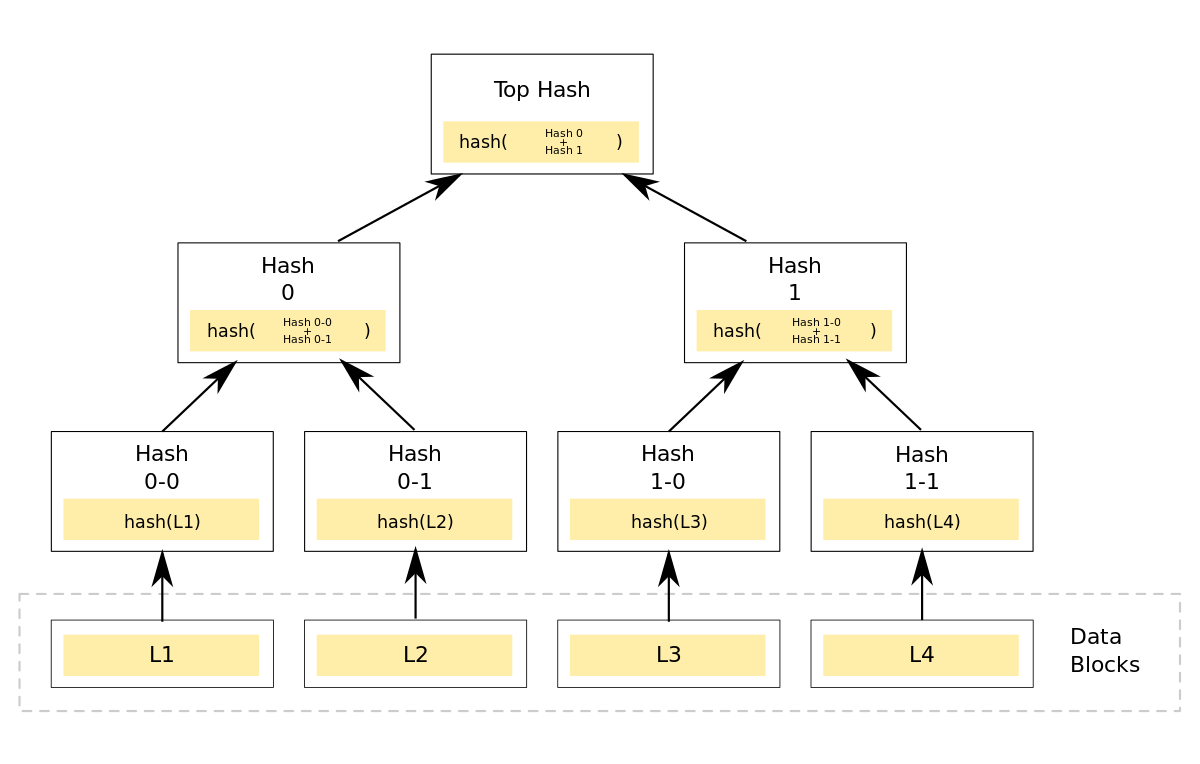
\includegraphics[width=1\columnwidth]{merkleTree}
	\captionsource{Merkle tree construction}{Merkle tree construction}
	{\url{https://en.wikipedia.org/wiki/Merkle_tree}}
	\label{fig:merkleTree}
\end{figure}

Given the top hash, known as the Merkle root, and a leaf, it is possible to prove the
membership by giving the path for each complementary hash. For example, given the
Merkle root and \texttt{L1}, the proof is \texttt{Hash 0-1} and \texttt{Hash 1}.
The verifier can then compute the hash of \texttt{L1}, the result of this hash
with \texttt{Hash 0-1}, and then with \texttt{Hash 1}. If the result is the same
as the Merkle root, then \texttt{L1} is a part of the tree.

In a block, the miner creates a Merkle tree of all included transaction
identifiers and puts the Merkle root into the header of the block. To validate
if a transaction is included in a block the path must be provided. Then the
resulting hash is compared to the Merkle root registered in the block's header.
\gls{spv} nodes, nodes without the full blockchain, download only block headers
and ask other nodes to provide partial views of relevant parts of the blockchain.

% -----------------------------------------------------------------------------
\section{Transactions}

Transactions allow users to move bitcoins from one address to another and are
the content of  Bitcoin's blockchain. In Bitcoin, the blockchain does
not store a balance for each user; the blockchain keeps only the history of all
transactions made since the beginning.

\subsection{A list of inputs \& outputs}

A transaction is composed of a list of inputs and a list of outputs. In other
words, where the bitcoins come from and where they go. An input refers to an
unspent output at the address from where funds will be spent, and output
refers to an address where the funds will go.  To spend funds the user needs
to control the addresses where unspent outputs are present. These unspent outputs are
called Uspent Transaction Output (\texttt{UTXOs}) and, combined, represent the total amount owned by a user.

\begin{figure}[H]
	\centering
	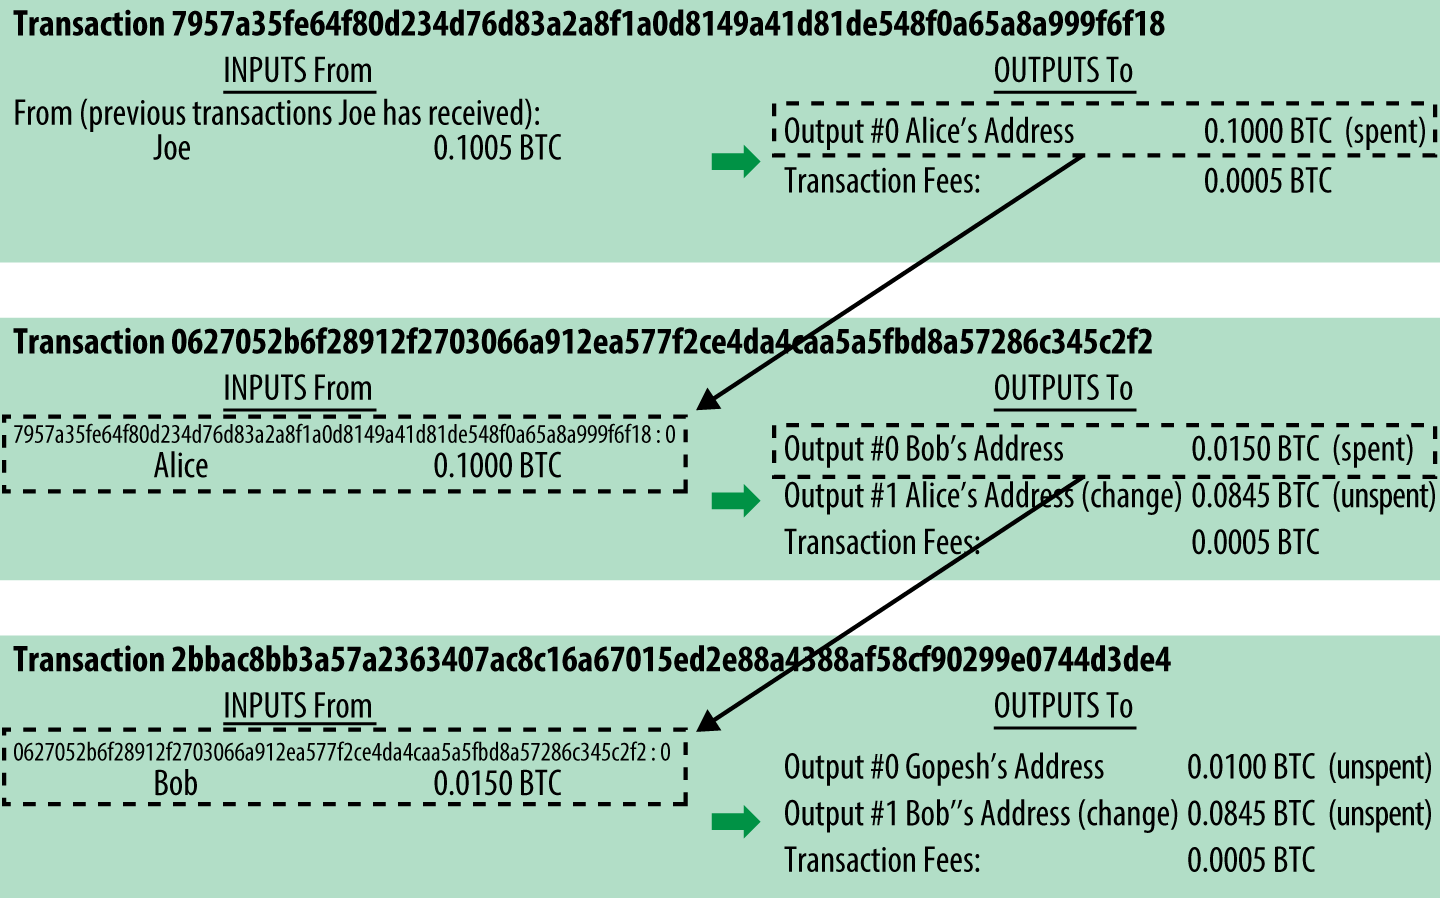
\includegraphics[width=1\columnwidth]{utxosChain}
	\captionsource{A chain of transactions where inputs and outputs are linked}
  {A chain of transactions where inputs and outputs are linked}
	{\url{https://github.com/bitcoinbook/bitcoinbook/blob/second_edition/ch02.asciidoc}}
	\label{fig:utxosChain}
\end{figure}

Each input has a value, the value specified in the output to which
the input points. The sum of the value of all inputs in a transaction must be more than the
sum of the values specified in the outputs, with the difference being the fee, meaning an input must be spent entirely.

The most straightforward transaction is composed of one input and one output
with the same amount of money in and out if we include the fee. However, the most typical transaction
is composed of one input, referring to where the funds come from, and two
outputs as it is rare to have the right amount available in one
\texttt{UTXO}. In this case, the first output is the user who will receive the funds, with
the amount transferred, and the second output is another address owned by the
sender to gather the change, i.e., the remaining amount.

As with blocks, transactions also have an identifier. These identifiers are created in the
same way as blocks, by taking the double hash of the data, i.e., the whole
transaction. This means that, in the original design, a transaction does not
have its final transaction identifier (TXID) before it is wholly signed, i.e., every
input.

\subsection{Transaction fees}

The sum of all inputs of a transaction constrains the sum of the
outputs, and the difference is implicitly considered as a fee (as
shown in Figure~\ref{fig:utxosChain}.) Fees were not required in the beginning, but
today a transaction will not be relayed, nor included in a block without paying fees. A
miner, when he finds a block, can create the first transaction without inputs,
where a fixed amount of new coins is created plus the total amount of fees
collected in all the included transactions. A miner will, therefore, select the
transactions that pay the most fees given the space they consume in the block.
Fees are calculated with the virtual size of the transaction, the virtual size is equal to
the transaction size in bytes. A ratio of fee per virtual byte is then selected
to find the fee for a transaction.

\subsection{Scripting language}

As described before, outputs or \texttt{UTXOs} are related to addresses and
proof of ownership is required to spend them. To spend a \texttt{UTXO}, the
Bitcoin protocol uses digital signatures, a valid
signature for the address from which the output is being spent is required and,
to sign, the private key is required. Thus, while signing a transaction
corresponding to the right address, it is possible to prove that the user owns
the address. However, the protocol does not just require signatures and public
keys, conditions to \textit{unlock} a \texttt{UTXO} are structured in scripts.
Bitcoin has a stack-based script language called \say{Bitcoin Script}.

\begin{figure}[H]
	\centering
	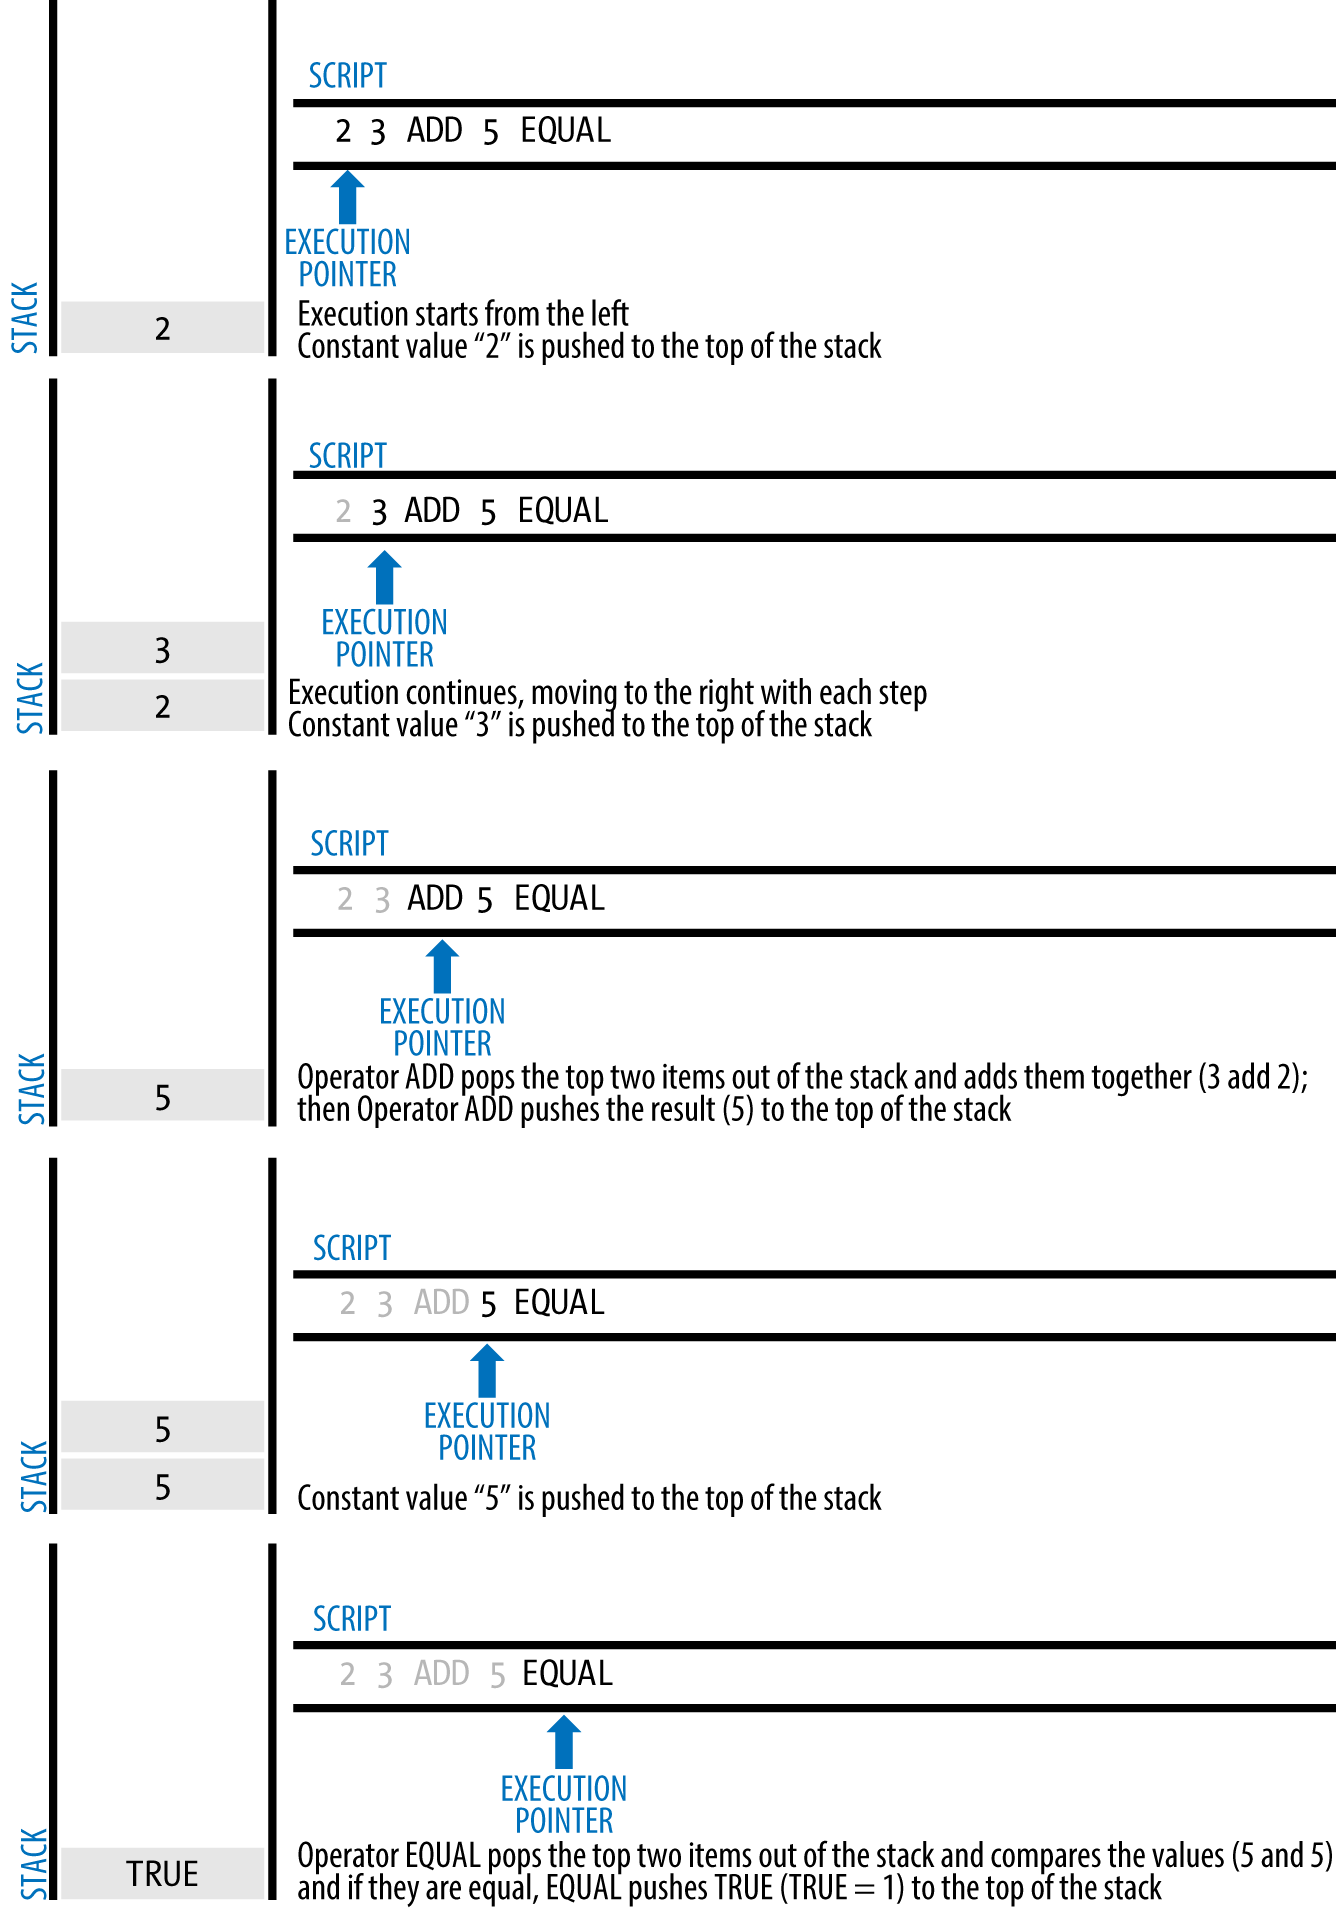
\includegraphics[width=0.73\columnwidth]{stackBased}
	\captionsource{Example of simple Bitcoin script program execution}
  {Example of simple Bitcoin script program execution}
	{\url{https://github.com/bitcoinbook/bitcoinbook/blob/second_edition/ch06.asciidoc}}
	\label{fig:stackBased}
\end{figure}

The list of all the \texttt{OP\_CODES} available in Bitcoin's scripting language
is in the documentation. Among them are \texttt{OP\_CHECKSIG}, which verifies a given
signature with a public key provided on top of the stack, \texttt{OP\_IF, OP\_ELSE,
OP\_ENDIF} create execution branches with a boolean on top of the stack,
\texttt{OP\_DUP} duplicates the value on top of the stack or \texttt{OP\_HASH160,
OP\_SHA256} which compute hashes of values on top of the stack.

Each input and output have a script. For outputs, the script establishes the
requirement to be fulfilled in order to be able to spend it. An address is the result
of the public key hashed with a \texttt{SHA256} and then hashed with a
\texttt{RIPEMD160} encoded with a checksum in a more human-readable format. A
user can decode the human-readable format of an address to retrieve the hash
and create an output script called \gls{p2pkh}. With the script, the
address is retrieved, and given the address and the script, only the user who
holds the private key of that address will be able to sign the transaction and
spend the funds. The user controlling that address can create a transaction where that
input points to the \texttt{UTXO} and, to unlock the funds, the user needs to sign
the transaction and give the signature with the public key in the input's
unlocking script. Before including a transaction in a candidate block, a miner
validates all the inputs. He needs to check if the outputs are in fact
\texttt{UTXOs}, so ensuring the outputs are \textit{unspent}, and execute the
unlocking script with the locking script. Both scripts are concatenated to
validate input; the unlocking script first, as shown in
Figure~\ref{fig:lockUnlock}.

\begin{figure}[H]
	\centering
	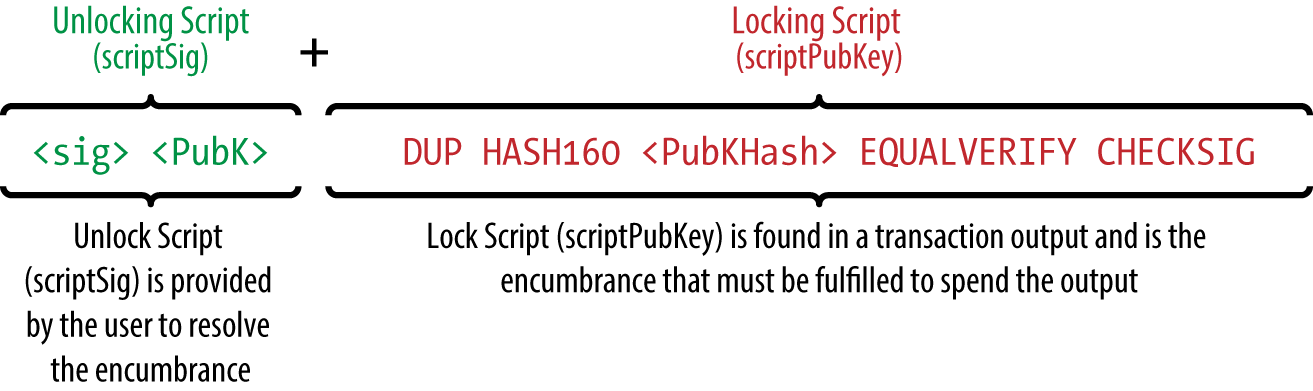
\includegraphics[width=1\columnwidth]{lockUnlock}
	\captionsource{Example of pay to public key hash script}
  {Example of pay to public key hash locking script with unlocking script}
	{\url{https://github.com/bitcoinbook/bitcoinbook/blob/second_edition/ch06.asciidoc}}
	\label{fig:lockUnlock}
\end{figure}

The script in Figure~\ref{fig:lockUnlock}, when executed, puts the signature on
top of the stack, then the public key. The public key is duplicated, hashed,
and the public key hash present in the locking script is put on top of the stack,
then the two first elements on top of the stack are then compared. If the
comparison fails, the script fails and the transaction is rejected. If the
test passes, the signature will be checked with the two remaining parameters on
the stack (i) the public key and (ii) the signature. If the signature is valid, the
value \texttt{True} is put on top of the stack. Otherwise, the
value \texttt{False} put on top of the stack. If the value \texttt{True} is present
on top of the stack at the end of the script the transaction is valid,
otherwise the transaction is invalid.

\gls{p2sh} is the second standard script mostly used. It provides the ability
to send outputs to a custom script without knowing the content of the script.
A user can create a custom script and give the hash of this script, encoded in an address,
to another user. When the output is spent the whole script must be provided in
the unlocking script. \gls{p2sh} are used, for example, to create multi-signature scripts.

\subsection{Segregated witness}

\gls{segwit} is the \gls{bip}141 that proposed changing the transaction
structure to fix transaction malleability, add script versioning, and improve
other aspects \cite{SegWit, SegWitBIP}. In fact, \gls{segwit} changed the way
outputs are structured. The malleability is fixed if all inputs use \gls{segwit}
only. A transaction can have \gls{segwit} inputs and non-\gls{segwit} inputs at
the same time. The \gls{bip} abstract explains its purpose:

\begin{quote}
  This BIP defines a new structure called a \say{witness} that is committed to
  blocks separately from the transaction merkle tree. This structure contains
  data required to check transaction validity but not required to determine
  transaction effects. In particular, scripts and signatures are moved into this
  new structure.

  The witness is committed in a tree that is nested into the block's existing
  merkle root via the coinbase transaction for the purpose of making this BIP
  soft fork compatible. A future hard fork can place this tree in its own branch.
\end{quote}

With \gls{segwit}, a transaction has two TXIDs. The first is determined without
all the witness data, so it is deterministic at transaction creation. The
second one is related to the witness data and changes when signatures appear.
This separation fixes the transaction malleability issue. The second big change is the
way the weight is calculated to determine the fees. The transaction weight
\texttt{Tx Weight} becomes $\texttt{Base Tx} * 3 + \texttt{Total Size}$ where
\texttt{BaseTx} is the size without the witness data and \texttt{Total Size} is
the serialized transaction with all the data, including the witness data. This new structure introduces a
virtual transaction size such that virtual size is equal to $\texttt{Tx Weight} /
4$. Thus, \gls{segwit} reduces the weight of the witness data in the calculus of
the fees.

\subsection{Transaction malleability}

The fact that the transaction identifier depends on the hash of the whole
serialized transaction while the signature does not currently cover all the data
in a transaction introduces what is called transaction malleability. A miner
could tweak the transaction to change is identifier before including it into a
block without invalidating it nor changing the claiming output conditions. This
malleability means that an unconfirmed chain of transactions must not be trusted
(because the following transactions will depend on the hashes of the previous
transactions.)

The first way to achieve malleability is to tweak the signatures themselves. For
every signature $(r, s)$, the signature $(r, -s \pmod n)$ is a valid signature
for the same message. As mentioned in the Bitcoin wiki about transaction
malleability:

\begin{quote}
	As of block 363724, the BIP66 soft fork has made it mandatory for all new
	transactions in the block chain to strictly follow the DER-encoded ASN.1 standard.
	Further efforts are still under way to close other possible malleability within
	DER signatures.
\end{quote}

However, even if the format is standardized and enforced, signatures can still
be changed by anyone who has access to the corresponding private keys. When the
user signs a transaction, the unlocking script (scriptSig) contains, e.g., for a
standard \gls{p2pkh}, the signature and the public key. These data are present
in the signed transaction, but cannot be present during the signing process
because they do not yet exist. This presence of signatures in the script means
that the content of unlocking scripts are not part of the signing data, but part
of the hashing data for the TXID. E.g., by introducing an additional
\texttt{OP\_CODE}, it is possible to change the TXID without invalidating the
signature.

Nevertheless, with \gls{segwit} activated, now the transaction malleability with
signatures and scripts is no longer possible. As mentioned in the \gls{bip} 141:

\begin{quote}
	It allows creation of unconfirmed transaction dependency chains without
	counterparty risk, an important feature for offchain protocols such as the
	Lightning Network.
\end{quote}


% -----------------------------------------------------------------------------
\section{Scalability of Bitcoin}

Improvements in the consensus layer have been made and will continue to appear
to answer the problem of scalability. However, modifying the consensus layer is
not easy, usually soft forks are needed, and in some cases hard forks, both of which
can be a lengthy and painful process as majority adoption of the changes is required. With
\gls{segwit}, the latest significant improvement on-chain, all the prerequisites
to construct a robust layer-two application, such as fixing malleability, are
fulfilled.

\subsection{Layer-two applications}

The layer-two is an architectural concept where a blockchain is used as a source
of truth and only for resolving disagreements. Usually, the construction that
uses this architectural concept is called payment channels or micropayment
channels. These channels enable scalability because they reduce the number of
transactions needed on the blockchain if two users exchange often.
Channels allow more than scalability, as payment channel transactions are
instant and can be accepted as \textit{confirmed} without latency. Latency is a
consequence of the mechanism that resolves the \textit{double-spending} problem
when funds are spent twice to different users. Payment channels create a
structure that ensures that no double-spending is possible for the funds locked
in the channel.

\chapter{Payment channels, a micropayment network}
\label{chap:paymentChannels}

Payment channels or micropayment channels, as mentioned previously, are one part
of the scalability solution. The idea of payment channels was suggested by
Satoshi in an email to Mike Hearn. Since then, various schemes to construct
such structures have been proposed. To have a better understanding of the
differences between various channel schemes, and to be able to analyze a channel
scheme objectively, a few formal definitions are needed. A list of formal definitions for
payment channel construction is proposed. An analysis of different commonly
exposed payment channel constructions is done following these definitions. The
list does not contain all the payment channel schemes, some of them
might be missing. However, the list contains a fairly good representation of the
different existing constructions.

Schemes can be optimized when a provider has multiple clients through multiple
channels. In this scenario the core feature is to be as cheap as possible for
the provider while being flexible for settlement. This specific case has been
explored through a white paper present in the following appendices. The content
of the white paper is summarized following the analysis.

Channels can be optimized with threshold cryptography. In fact, the amount
economized can be significative according to the cases. An analysis is performed
to define, with and without \gls{segwit}, possible savings for
payment channel transactions.

\minitoc

\newpage

% -----------------------------------------------------------------------------
\section{Formal definitions}

These formal definitions specify the necessary and sufficient conditions for a
payment channel to be qualified as a member of a specific set. They set boundaries or limits that separate
the term from any other term. The following formal definitions qualify
properties that micropayment channels based on a blockchain such as Bitcoin can
have with the view of a particular player. Transactions represent a set of
information with a special meaning for the given blockchain that modify the
channel state. A transaction can be broadcast to the network to effectively
affect the on chain channel state or been kept by the player. Players are users of the
given blockchain and they own funds. Funds are owned by one and only one
player at a time. The meaning of owning an amount of funds in a channel for a given player is defined as holding a transaction not yet broadcast that allows this player to claim this amount of funds.

\begin{definition}[Trustless]
  A channel is trustless for a player $p_i \in \mathcal{P} = \{\mathcal{P}_0,
  \dots, \mathcal{P}_n\}$ if and only if the safety of his funds at each step
  $\mathcal{S}$ of the protocol does not depend on the behavior of players $\mathcal{P}' =
  \mathcal{P} - p_i$.
\end{definition}

\begin{definition}[Optimal]
  A channel is optimal for a player $p_i \in \mathcal{P} = \{\mathcal{P}_0, \dots,
  \mathcal{P}_n\}$ if and only if the number of transactions
  $\mathcal{T}(\mathcal{C})$ needed to claim the funds for a given constraint
  $\mathcal{C}$ is equal to the number of moves $\mathcal{M}(\mathcal{C})$ needed
  to satisfy the constraint at any time.
\end{definition}

For example, for a refund constraint $\mathcal{C}$ in a channel $\mathcal{P}_1 \rightarrow \mathcal{P}_2$,
refunding $\mathcal{P}_1$ requires $\mathcal{M}(\mathcal{C}) = 1$, thus
an optimal scheme requires $\mathcal{T}(\mathcal{C}) = \mathcal{M}(\mathcal{C}) = 1$.

\begin{definition}[Open-ended]
  A channel is open-ended for a player $p_i \in \mathcal{P} = \{\mathcal{P}_0,
  \dots, \mathcal{P}_n\}$ if and only if there is no predetermined channel
  lifetime at the setup.
\end{definition}

A channel that is not open-ended can have a mechanism to refresh the channel
on-chain with a designated transaction before the end of the lifetime.

\begin{definition}[Undelayed]
  A channel is undelayed for a player $p_i \in \mathcal{P} = \{\mathcal{P}_0,
  \dots, \mathcal{P}_n\}$ if and only if this player can broadcast their set of
  transactions at any time.
\end{definition}

\begin{definition}[Non-interactive]
  A channel is non-interactive for a player $p_i \in \mathcal{P} =
  \{\mathcal{P}_0, \dots, \mathcal{P}_n\}$ if and only if this player does not
  have the responsibility to watch the targeted blockchain to react to arbitrary events $\mathcal{E}$ in order to guarantee their safety.
\end{definition}

With these five definitions, it is possible to infer a significant necessary
corollary. If a channel is undelayed for a player this player can broadcast his
latest state without constraint, and if this channel is also optimal for the
same player only one transaction is needed to move the funds. If only one
transaction is needed to move the funds, then the funds are directly available
for this player. If the funds are available instantly, then the channel is
instantaneous for the player.

\begin{corollary}[Instantaneous]
  A channel is instantaneous for a player $p_i \in \mathcal{P} = \{\mathcal{P}_0, \dots,
  \mathcal{P}_n\}$ if and only if the channel is undelayed and optimal for this
  player.
\end{corollary}

\subsection{Types of payment channel}

We can distinguish two type of channels, unidirectional channels that allow
one user to send money to another user and bidirectional
channels that allow two users to send in either direction. Usually, a
bidirectional channel is more optimal than two unidirectional channels but
introduces other constraints.

\subsubsection{Unidirectional}

In a two-player unidirectional channel, there is a payer, later referred to as
player-one or client, and a payee, later referred to as player-two or provider.
It is not possible to transfer money back in the reverse direction in the
channel. These channels are asymmetric, each player benefits from different channel
properties. The analysis must be done in the view of each player $p_i \in
\mathcal{P} = \{\mathcal{P}_0, \dots, \mathcal{P}_n\}$ at a time.

\subsubsection{Bidirectional}

In a two-player bidirectional channel $\mathcal{C}$, the player $A$ and the
player $B$ can send funds in direction $\mathcal{C}_{AB}$ and
$\mathcal{C}_{BA}$. A bidirectional channel can be a specific scheme or a
pairing of existing unidirectional channels. These channels are generaly
symmetric, each player $p_i \in \mathcal{P} = \{\mathcal{P}_0, \dots,
\mathcal{P}_n\}$ benefits from the same channel properties.

\section{Analysis of payment channels}

\subsection{Spilman-style payment channels}

Spilman-style payment channels, proposed by Jeremy Spilman in 2013
\cite{SpilmanStyle}, are the most simple construction of a unidirectional
payment channel. They have a finite lifetime predefined at the setup phase and
the client, i.e., the payer, cannot trigger their refund before the end of the
channel lifetime (but he can receive his funds back if the payee settles the
channel before the end of the lifetime.) The channel is one-time use. When the
payer or the payee get their funds, the channel is closing. Neither the payer nor the
payee need to watch the blockchain to react to events during the lifetime of
the channel because only the payee can broadcast a transaction, so both do not
need to watch the blockchain to be safe. It is worth noting that, without a
proper fix to transaction malleability \cite{SegWitBIP, BIP62,
DBLP:journals/corr/AndrychowiczDMM13, DBLP:journals/corr/DeckerW14}, this scheme
is not secure.

\begin{table}[h]
  \begin{tabularx}{\textwidth}{ | X | l | l | l | l | l |}
  \hline
  Player & Trustless & Optimal & Open-ended & Undelayed & Non-interactive \\ \hline \hline
  Payer & Yes & Yes & No & No & Yes \\ \hline
  Payee & Yes & Yes & No & Yes & Yes \\
  \hline
  \end{tabularx}
  \caption{Summary of Spilman-style payment channel properties}
  \label{fig:summarySpilmanPaymentChannel}
\end{table}

According to the previous definitions, Spilman-style ephemeral payment channels are
instantaneous non-interactive channels for the payee, and optimal non-interactive for
the payer.

\subsection{\texttt{CLTV}-style payment channels}

Introduced in 2015, \texttt{CLTV}-style payment channels are a solution to the malleability
problem in Spilman-style payment channels. With the new \texttt{OP\_CODE} check
locktime verify (\texttt{OP\_CHECKLOCKTIMEVERIFY}), redefining the
\texttt{OP\_NOP2}, it is possible to enforce the non-spending of a transaction
output until some time in the future. With \texttt{OP\_CHECKLOCKTIMEVERIFY} a
transaction output can enforce the spending transaction to have a
\texttt{nLockTime} later or equal to the specified value in the script
\cite{BIP65}.

Instead of creating a funding transaction and a refund transaction vulnerable to
transaction malleability attacks, the client creates the funding transaction
output with a script (Listing~\ref{lst:scriptPubKeyCLTV}) that allows the
provider and the client to spend the funds
with co-operation or after a lock time the client can spend the funds without
the co-operation of the provider.

\begin{listing}
  \begin{minted}[breaklines=true,fontsize=\scriptsize]{text}
IF
    <provider pubkey> CHECKSIGVERIFY
ELSE
    <expiry time> CHECKLOCKTIMEVERIFY DROP
ENDIF
<client pubkey> CHECKSIG
  \end{minted}
	\caption{Locking script (scriptPubKey) with \texttt{CHECKLOCKTIMEVERIFY}}
	\label{lst:scriptPubKeyCLTV}
\end{listing}

\texttt{CLTV}-style payment channels have the same properties as Spilman-style payment
channels following the previous definitions but are not subject to transaction
malleability attacks.


\subsection{Decker-Wattenhofer duplex payment channels}

Decker-Wattenhofer duplex payment channels \cite{Decker2015fast}, also called
\gls{dmc}, proposed in 2015, are bidirectional channels based on pairs of
Spilman-style unidirectional channels. The construction has a finite lifetime
predefined at the setup phase but can be refreshed on-chain to keep the channel
open with an updated state. During the refresh process, it is possible to refill
the channel, and the scheme allows payment routing with \gls{htlc}.

\gls{dmc} payment channels are not optimal. Uncooperative closing of the channel
requires $d + 2$ transactions (where $d$ is equal to the revocation tree depth).
They are not undelayed, without other players cooperation the funds are
recovered after \texttt{nLockTime} values. \gls{dmc} are not open-ended, a
dedicated transaction needs to be broadcast before the end of the
\texttt{nLockTime}.

\begin{table}[h]
  \begin{tabularx}{\textwidth}{ | X | l | l | l | X |}
  \hline
  Trustless & Optimal & Open-ended & Undelayed & Non-interactive \\ \hline \hline
  Yes & No & (Yes) & No & No \\
  \hline
  \end{tabularx}
  \caption{Summary of Decker-Wattenhofer duplex payment channel properties}
  \label{fig:summaryDeckerWattenhoferPaymentChannel}
\end{table}

\subsection{Poon-Dryja payment channels}

Poon-Dryja payment channels, also called Lightning Network, is a proposed
implementation of \gls{htlc} with bidirectional payment channels which allow
payments to be securely routed across multiple peer-to-peer payment channels
\cite{poon2016bitcoin}.

\begin{table}[h]
  \begin{tabularx}{\textwidth}{ | X | l | l | l | X |}
  \hline
  Trustless & Optimal & Open-ended & Undelayed & Non-interactive \\ \hline \hline
  Yes & No & Yes & Yes & No \\
  \hline
  \end{tabularx}
  \caption{Summary of Poon-Dryja payment channel properties}
  \label{fig:summaryPoonDryjaPaymentChannel}
\end{table}

Their scheme is trustless (assuming that \gls{segwit} has been implemented),
open-ended, and undelayed but not optimal when the channel closes without
co-operation nor non-interactive.

\subsection{Summary}

\begin{table}[h]
  \begin{tabularx}{\textwidth}{ | X | l | l | l | l | l |}
  \hline
  Channel & Type & Optimal & Open-ended & Undelayed & Non-inter. \\ \hline \hline
  Spilman-style & Uni & Yes/Yes & No/No & No/Yes & Yes/Yes \\ \hline
  CLTV-style & Uni & Yes/Yes & No/No & No/Yes & Yes/Yes \\ \hline
  Decker-Wattenhofer \gls{dmc} & Bi & No & (Yes) & No & No \\ \hline
  Poon-Dryja & Bi & No & Yes & Yes & No \\ \hline
  Shababi-Gugger-Lebrecht & Uni & No/Yes & Yes/Yes & No/Yes & Yes/No \\
  \hline
  \end{tabularx}
  \caption{Summary of different payment channels}
  \label{fig:summaryPaymentChannel}
\end{table}

This table summarizes the different properties of the proposed definitions of
common channel schemes. The last row refers to the next presented scheme.

% -----------------------------------------------------------------------------
\section{One-way channel (Shababi-Gugger-Lebrecht)}

Our one-way payment channel for Bitcoin is a modified version of other layer-two
applications, such as \say{Yours Lightning Protocol} or Lightning Network
\cite{poon2016bitcoin, YoursLightningProtocol}. The scheme is specially designed
for a client to provider scenario, where the provider has multiple clients
through multiple channels. The core design aims to be as cheap as possible for
the provider while being flexible for settlement. The white paper \say{Partially
Non-Interactive and Instantaneous One-way Payment Channel for Bitcoin} inserted
after the appendices, describes the core design and the incentives.

\begin{table}[h]
  \begin{tabularx}{\textwidth}{ | X | l | l | l | l | l |}
  \hline
  Player & Trustless & Optimal & Open-ended & Undelayed & Non-interactive \\ \hline \hline
  Payer & Yes & No & Yes & No & Yes \\ \hline
  Payee & Yes & Yes & Yes & Yes & No \\
  \hline
  \end{tabularx}
  \caption{Summary of Shababi-Gugger-Lebrecht payment channel properties}
  \label{fig:summaryShababiGuggerLebrechtPaymentChannel}
\end{table}

A part of this thesis was devoted to writing the white paper describing our
channel scheme while working on the scheme itself. During this work we found a
possible attack described in the white paper which we fixed.

The next step has been to analyze how it is possible to optimize the channel
with threshold cryptography. As it is possible to see, every channel
construction depends on a funding transaction that locks funds in a 2-out-of-2
multi-signature script. This funding transaction is always on-chain, so if it is
possible to replace this \gls{p2sh} with a standard \gls{p2pkh} output the savings
should be attractive.


% -----------------------------------------------------------------------------
\section{Optimizing payment channels}

Three transactions are compared with \gls{segwit}\footnote{ The transaction size
is calculated with nested-\gls{segwit} and not with native mode.} and without.
Optimization is expressed in percentage of size or virtual-size economized. The
Script Hash (SH) consumes a multi-signature script, and the Public Key Hash
(PKH) consumes a standard public key. Note that size can vary by a few bytes with
\gls{segwit}.

% ** P2SH
% |               | segwit | segwit | non-segwit | non-segwit |
% |               |   size |  vsize |       size |      vsize |
% |---------------+--------+--------+------------+------------|
% | first refund  |    340 |    174 |        302 |        302 |
% | refund normal |    372 |    207 |        335 |        335 |
% | settlement    |    372 |    207 |        335 |        335 |
%
% ** PKH
% |               | segwit | segwit | non-segwit | non-segwit | native segwit | native segwit |
% |               |   size |  vsize |       size |      vsize |          size |         vsize |
% |---------------+--------+--------+------------+------------+---------------+---------------|
% | first refund  |    216 |    134 |        191 |        191 |           192 |           110 |
% | refund normal |    246 |    165 |        226 |        226 |           224 |           142 |
% | settlement    |    246 |    165 |        226 |        226 |           224 |           142 |

\newcolumntype{S}{>{\hsize=.5\hsize}C}
\begin{table}[h]
  \begin{tabularx}{\textwidth}{| X | S | S | S | S | S | S |}
  \cline{3-7}
  \multicolumn{2}{l|}{ } & \multicolumn{2}{c|}{Non-\gls{segwit}} & \multicolumn{3}{c|}{\gls{segwit}} \\ \hhline{~~-----}
  \multicolumn{2}{l|}{ } & R-Size & O & \cellcolor[gray]{0.9} R-Size & V-Size & O \\ \hhline{--=====}
  \multirow{2}{*}{First Refund}  & SH   & 302  & \multirow{2}{*}{36.75\%} & \cellcolor[gray]{0.9} 340 & 174  & \multirow{2}{*}{22.99\%} \\ \hhline{~--~--~}
                                 & PKH  & 191  &                          & \cellcolor[gray]{0.9} 216 & 134  &                          \\ \hhline{-------}
  \multirow{2}{*}{Refund Normal} & SH   & 335  & \multirow{2}{*}{32.54\%} & \cellcolor[gray]{0.9} 372 & 207  & \multirow{2}{*}{20.29\%} \\ \hhline{~--~--~}
                                 & PKH  & 226  &                          & \cellcolor[gray]{0.9} 246 & 165  &                          \\ \hhline{-------}
  \multirow{2}{*}{Settlement}    & SH   & 335  & \multirow{2}{*}{32.54\%} & \cellcolor[gray]{0.9} 372 & 207  & \multirow{2}{*}{20.29\%} \\ \hhline{~--~--~}
                                 & PKH  & 226  &                          & \cellcolor[gray]{0.9} 246 & 165  &                          \\ \hhline{-------}
  \end{tabularx}
  \caption{Summary of transaction size optimization}
  \label{fig:summaryTransactionSizeOpti}
\end{table}

The average fee per virtual byte in the last three months was around 292 Satoshis. This
optimization allows savings of up to 32,412 Satoshis for the first refund
transaction without \gls{segwit}, and 12,264 Satoshis for a refund or a
settlement transaction with \gls{segwit}. At the current price, these savings
represent between USD \$1.31 and USD \$3.47\footnote{ Average price of Bitcoin
in the last 3 months, around \$10,700 USD}. If the channel is
used for micropayments such as a couple of cents each time, this optimization
makes a difference and lowers the required threshold for feasibility. The first
refund transaction being less expensive also makes the clients commitment
easier. The Table~\ref{fig:summaryTransactionSizeOpti} exhibits transaction
utilizing only one input, and it is worth noting that the number of input has a
supralinear influence to the savings.

Requirements need to be defined to be able to substitute the multi-signature script
with a threshold scheme. Analysis of the protocol and the signing process for a
multi-signature script allows one to define these requirements. A 2-out-of-2 multi-signature
script can be unlocked with two different public keys and their signature. The
signing order only matters in that it is determined at the time of creating a
multisig address. Some standards such as \gls{bip}45 address the need to
predefine or communicate the ordering of the keys (and therefore the signatures)
by always ordering the keys lexicographically, and always ordering the
signatures in order of the keys \cite{BIP45}.
The protocol takes advantage of this fact. A transaction is usually held fully signed
only by one player. The threshold scheme must follow these requirements (i) 2
players need to co-operate to generate a valid signature, (ii) both must be able
to start the signing process, and (iii) only one player must be able to retrieve
the signature at the end of the process. If both need the signature it is
always feasible to share, meaning the current protocol is not better in this case.

\chapter{ECDSA asymmetric threshold scheme}
\label{chap:threshold}

Threshold cryptography has been discussed for a long time already, many
cryptographic schemes like RSA or Paillier \cite{10.1007/BFb0052253,
10.1007/978-3-642-27954-6_20} exists, but the difficulty is to use them in real
case application. Since Bitcoin become famous, people lose funds because they
lost keys or get hacked. Since then research has been done to secure Bitcoin
wallets \cite{Goldfeder2015SecuringBW, DBLP:conf/acns/GennaroGN16}. However, the
most significant problem today in Bitcoin that slow down the adoption of
threshold cryptosystem is the complexity of creating an efficient and flexible
scheme for \gls{ecdsa}. Recently, researchers focused on finding more efficient
and more generic system, but fortunately, a protocol fulfilling perfectly the
needs described in the previous chapter required to improve payment channel in
Bitcoin already exists. Nevertheless, this scheme explains how to perform a
\gls{dsa} threshold signature and not \gls{ecdsa}. So the protocol needs to be
adapted.

The scheme analyzed, transformed, and implemented in the following has been
proposed by MacKenzie and Reiter in their paper \say{Two-Party Generation of DSA
Signatures} \cite{crypto-2001-1592}. This scheme is also the basis of several
other papers cited before. They base their construction of a threshold signature
scheme with \gls{dsa} based on a simple multiplicative shared secret and
homomorphic encryption to keep the individual values unknown by the other
player. The homomorphic encryption used as an example in the paper and chose for
the implementation is the Paillier cryptosystem
\cite{Paillier:1999:PCB:1756123.1756146}. The following chapter describes how to
adapt the scheme form \gls{dsa} to \gls{ecdsa} and introduce some fundamental
building blocks needed for a real case scenario like hierarchical deterministic
threshold wallet or deterministic signatures.

\minitoc

\newpage

% -----------------------------------------------------------------------------
\section{Reminder}

Before introducing the threshold scheme, reminders of basic components used in
the scheme are presented. This reminders are composed of \gls{ec} basic
mathematics, Paillier homomorphic encryption scheme, and digital signature
protocols, in particular \gls{dsa} and \gls{ecdsa}.

\subsection{Elliptic curves}

Bitcoin use \gls{ec} cryptography for securing his transaction. \gls{ecdsa},
based on the \gls{dsa} proposal by the \gls{nist}, over the curve secp256k1,
proposed by the \gls{secg}, is used \cite{sec2}.

\subsubsection{Secp256k1 curve}

The curve secp256k1 is define over the finite field $\mathbb{F}_p$ of $2^{256}$
bits with a Koblitz curve $y^2 = x^3 + ax + b$ where $a = 0$ and $b = 7$.
\begin{equation*}
\begin{split}
  y^2 &= x^3 + 7\\
\end{split}
\end{equation*}
\begin{equation*}
\begin{split}
  p &= &\text{\scriptsize FFFFFFFF FFFFFFFF FFFFFFFF FFFFFFFF FFFFFFFF FFFFFFFF FFFFFFFE FFFFFC2F}\\
  G &= &\text{\scriptsize (79BE667E F9DCBBAC 55A06295 CE870B07 029BFCDB 2DCE28D9 59F2815B 16F81798,}\\
    &  &\text{\scriptsize  483ADA77 26A3C465 5DA4FBFC 0E1108A8 FD17B448 A6855419 9C47D08F FB10D4B8)}\\
  n &= &\text{\scriptsize FFFFFFFF FFFFFFFF FFFFFFFF FFFFFFFE BAAEDCE6 AF48A03B BFD25E8C D0364141}
\end{split}
\end{equation*}

The curve order $n$ define the number of elements (points) generated by the
generator $G$ on the curve. Exponentiation of the generator $g^a \mod p$ become
a point multiplication with the generator $a \cdot G$.

\subsubsection{Points addition}
With two distinct points $P$ and $Q$ on the curve $\mathcal{E}$, geometrically
the resulting point of the addition is the inverse point, $(x, -y)$ of the
intersection point with a straight line between $P$ and $Q$. An infinity point
$\mathcal{O}$ represent the identity element in the group. Algebraically the
resulting point is obtained with:

\begin{equation}
\begin{split}
  P + Q &= Q + P = P + Q + \mathcal{O} = R \\
  (x_p, y_p) + (x_q, y_q) &= (x_r, y_r) \\
  x_r &\equiv \lambda^2 - x_p - x_q \pmod p \\
  y_r &\equiv \lambda(x_p - x_r) - y_p \pmod p  \\
  \lambda &= \cfrac{y_q - y_p}{x_q - x_p} \\
          &\equiv (y_q - y_p)(x_q - x_p)^{-1} \pmod p
\end{split}
\end{equation}

\subsubsection{Point doubling}

For $P$ and $Q$ equal, the formula is similar, the tangent to the curve
$\mathcal{E}$ at point $P$ determine $R$.

\begin{equation}
\begin{split}
  P + P &= 2P = R \\
  (x_p, y_p) + (x_p, y_p) &= (x_r, y_r) \\
  x_r &\equiv \lambda^2 - 2x_p \pmod p \\
  y_r &\equiv \lambda(x_p - x_r) - y_p \pmod p  \\
  \lambda &= \cfrac{3x_p^2 + a}{2y_p} \\
          &\equiv (3x_p^2 + a)(2y_p)^{-1} \pmod p
\end{split}
\end{equation}

\subsubsection{Point multiplication}

A point $P$ can be multiply by a scalar $d$. The straightforward way of
computing a point multiplication is through repeated addition where $dP = P_1 +
P_2 + \dots + P_d$.

% However, this is a fully
% exponential approach to computing the multiplication.
% The simplest method is the double-and-add method. To compute
% $dP = P_1 + P_2 + \dots + P_d$, start with the
% binary representation for $d : d = d_0 + 2d_1 + 2^2d_2 + \dots + 2^md_m$,
% where
% $[ d_0 \dots d_m] \in {0,1}$, $N = P, Q = \mathcal{O} \and \forall d_x : \text{if } d_x = 1 Q = \text{add}(Q, P), N = \text{double}(N)$.


\begin{lemma}[Elliptic Curve Discrete Logarithm Problem]
  Given a multiple $Q$ of $P$ where $Q = nP$ it is infeasible to find $n$ if $n$ is large.
\end{lemma}

\begin{lemma}[Point Order]
  A point $P$ has order $2$ if $P + P = \mathcal{O}$, and therefore $P = -P$.
  A point $Q$ has order $3$ if $Q+Q+Q=\mathcal{O}$, and therefore $Q + Q = -Q$.
\end{lemma}


\subsection{Paillier cryptosystem}

\begin{quote}{Wikipedia:}
  The Paillier cryptosystem, invented by and named after Pascal Paillier in 1999,
  is a probabilistic asymmetric algorithm for public key cryptography. The problem
  of computing $n$-th residue classes is believed to be computationally difficult.
  The decisional composite residuosity assumption is the intractability hypothesis
  upon which this cryptosystem is based.
\end{quote}

\subsubsection{Encryption}

With a public key $(n, g)$ and a message $m < n$, select a random $r < n$ and
compute the ciphertext $c = g^m \cdot r^n \mod n^2$ to encrypt the plaintext.

\subsubsection{Decryption}

With a private key $(n, g, \lambda, \mu)$ and a ciphertext $c \in
\mathbb{Z}_{n^2}^*$ compute the plaintext as $m = L(c^{\lambda} \mod n^2) \cdot
\mu \mod n$ where $L(x) = \frac{x-1}{n}$.

\subsection{Signature schemes}
\subsubsection{Digital Signature Algorithm}

\begin{quote}{Wikipedia:}
  The Digital Signature Algorithm (DSA) is a Federal Information Processing Standard
  for digital signatures. In August 1991 the National Institute of Standards and
  Technology (NIST) proposed DSA for use in their Digital Signature Standard (DSS)
  and adopted it as FIPS 186 in 1993.
\end{quote}

\paragraph{Signing}

With public parameters $(p, q, g)$, \texttt{hash} the hashing function,
$m$ the message, and $x \in \mathbb{Z}_q$ the private key.

\begin{itemize}
  \item Generate a random $k \in \mathbb{Z}_q$
  \item Calculate $r \equiv (g^k \pmod p) \pmod q : r \neq 0$
  \item Calculate $s \equiv k^{-1}(\texttt{hash}(m) + xr) \pmod q : s \neq 0$
  \item The signature is $(r, s)$
\end{itemize}

\paragraph{Verifying}

With public parameters $(p, q, g)$, \texttt{hash} the hashing function,
$m$ the message, $(r, s)$ the signature, and $y = g^x \mod p$ the public key.

\begin{itemize}
  \item Reject the signature if $r, s \notin \mathbb{Z}_q$
  \item Calculate $w \equiv s^{-1} \pmod q$
  \item Calculate $u_1 \equiv \texttt{hash}(m) \cdot w \pmod q$
  \item Calculate $u_2 \equiv rw \pmod q$
  \item Calculate $v \equiv (g^{u_1}y^{u_2} \pmod p) \pmod q$
  \item The signature is valide iff $v = r$
\end{itemize}

\subsubsection{Elliptic Curve Digital Signature Algorithm}

\gls{ecdsa} is a variant of \gls{dsa} which uses elliptic curve cryptography and
require a different set of parameters and smaller keys.

\paragraph{Signing}

With public parameters $(\mathcal{E}, G, n)$, \texttt{hash} the hashing function,
$m$ the message, and $x \in \mathbb{Z}_n$ the private key.

\begin{itemize}
  \item Generate a random $k \in \mathbb{Z}_n$
  \item Calculate $(x_1, y_1) = k \cdot G$
  \item Calculate $r \equiv x_1 \pmod n : r \neq 0$
  \item Calculate $s \equiv k^{-1}(\texttt{hash}(m) + xr) \pmod n : s \neq 0$
  \item The signature is $(r, s)$
\end{itemize}

\paragraph{Verifying}

With public parameters $(\mathcal{E}, G, n)$, \texttt{hash} the hashing function,
$m$ the message, $(r, s)$ the signature, and $Q = x \cdot G$ the public key.

\begin{itemize}
  \item Reject the signature if $r, s \notin \mathbb{Z}_n$
  \item Calculate $w \equiv s^{-1} \pmod n$
  \item Calculate $u_1 \equiv \texttt{hash}(m) \cdot w \pmod n$
  \item Calculate $u_2 \equiv rw \pmod n$
  \item Calculate the curve point $(x_1, y_1) = u_1 \cdot G + u_2 \cdot Q$ if
  $(x_1, y_1) = \mathcal{O}$ then the signature is invalid
  \item The signature is valide iff $r \equiv x_1 \pmod n$
\end{itemize}

\subsubsection{Schemes' analysis}

In $(r, s)$ the computation of the part $s$ remain the same in each signature
scheme, the only difference for $s$ is the modulus applied. In \gls{dsa} the
modulus $q$ is took, i.e. the order of the generator $g$ modulo $p$,  while in
\gls{ecdsa} the modulus $n$ is took, i.e. the order of the generator $G$ on the
curve $\mathcal{E}$.

The biggest adaptation is on how to calculate the part $r$ from the private
random $k$. In \gls{dsa} the generator $g$ is used with, at first, modulo $p$
and then modulo $q$ while in \gls{ecdsa} the curve is used. The signer generates
a  point and uses the coordinate $x_1$ modulo $n$.

\begin{postulate}
  This statement $a \equiv g^b \pmod p$ is equivalent in term of security to $a = b \cdot G$
  and $a \equiv (g^b \pmod p) \pmod q$ is equivalent to $a \equiv x \pmod n : (x, y) = b \cdot G$.
  \label{post:adaptEcdsa}
\end{postulate}

The previous postulate is used to adapt zero-knowledge proofs from \gls{dsa} to
\gls{ecdsa} hereafter. Lack of time has not permitted further researched this
postulate.


% -----------------------------------------------------------------------------
\section{Threshold scheme}

The \say{Two-party generation of DSA signatures} scheme presented by MacKenzie
and Reiter, as mentioned before, is an asymmetric scheme, i.e., at the end of
the protocol, only the initiator can retrieve the full signature. The scheme
proposed is a cryptographic (1,2)-threshold, i.e., one corrupted player can
occur on the two players, and the scheme remains safe. It is worth noting that
this is qualified as an optimal $(t, n)$-threshold scheme, i.e., $t = n - 1$
because if only one honest player remains the safety is guaranteed.

As also mentioned before, the scheme corresponds to the same requirement of a
Bitcoin 2-out-of-2 multi-signatures script. That means that it is possible to
use it to improve the payment channels. However, it is necessary to adapt the
scheme and particularly the zero-knowledge proofs construction. The following
explains the chosen adaptation.

The presented scheme in the original paper uses a multiplicative shared secret
and a multiplicative shared private random value. The secret $x$ is shared
between Alice and Bob, so that Alice holds the secret value $x_1 \in
\mathbb{Z}_{q}$ and Bob $x_2 \in \mathbb{Z}_{q}$ such that $x \equiv x_1x_2
\pmod q$. Along with the public key $y$, $y_1 \equiv g^{x_1} \pmod p$ and $y_2
\equiv g^{x_2} \pmod p$ are public. Alice holds a private key, from now on
mentioned as $sk$, corresponding to a public encryption key $pk$. Alice also
knows a public encryption key $pk'$ for which she does not know the private key
$sk'$. Here the Paillier homomorphic cryptosystem is used as the encryption
scheme, but it is worth noting that others homomorphic encryption systems can be
used to implement the scheme. Alice and Bob know a set of parameters used for
both zero-knowledge proofs.

Starting now the initialization is not taken into account, and the author
assumes that reader has a good understanding of the original scheme
\cite{crypto-2001-1592}. The choice was made to focus the amount of work on the
signing protocol and because the implementation is not directly part of the
cryptographic \texttt{C} library. This initialization can be further research
for another thesis.

\subsection{Adapting the scheme}

Except for the zero-knowledge proofs, the adaptation is trivial and require just
the same adaptation of the \gls{dsa} signature scheme and \gls{ecdsa} signature
scheme, i.e., compute the $r$ value with the curve. The following figures
describe the adapted scheme. The adapted protocol keeps the same messages, so
they are not repeated. The postulate~\ref{post:adaptEcdsa} is used to perform
the adaptation.

The secret remain shared multiplicatively so that so that Alice holds the secret
value $x_1 \in \mathbb{Z}_{n}$ and Bob $x_2 \in \mathbb{Z}_{n}$ such that $x
\equiv x_1x_2 \pmod n$. Alice holds her public key $Q_1 = x_1 \cdot G$ and Bob
$Q_2 = x_2 \cdot G$ such that $Q = x_1 \cdot Q_2$ for Alice or $Q = x_2 \cdot
Q_1$ for Bob. The notation $\cdot$ is used to denote the point multiplication
over \gls{ec}.

All the random values $k$ are chosen in $\mathbb{Z}_{n}$ instead of
$\mathbb{Z}_{q}$, also in the case of deterministic signature. All the
computation modulo $q$ is replaced by modulo $n$, as shown in the previous
digital signature recap. Values $R_2$ and $R$ become points. Verifications of
values $R_2$ and $R$ become point verifications on the curve and $r'$ is
calculated by Alice and Bob as shown in the other reminder. The value $cq$ added
to the homomorphic encrypted signature is transformed into $cn$ to hide values
$z_2$ and $x_2z_2$.

The author noticed an error of notation in the original paper. On the second
line Alice compute $z_1 \equiv (k_1)^{-1} \pmod n$ and the original paper use
the random value selection $\xleftarrow[]{R}$ instead of a standard assignation
$\leftarrow$. This error is corrected in the following version of the protocol.

\newpage

\begin{figure}[H]
    \begin{table}[H]
      \centering
      \begin{footnotesize}
      {\renewcommand{\arraystretch}{1.2}%
      \begin{tabular}{ | l l | }
        \hline
        \multicolumn{1}{|c}{alice}  & \multicolumn{1}{c|}{bob} \\
        $k_1 \xleftarrow[]{R} \mathbb{Z}_{n}$ & \\
        $z_1 \leftarrow (k_1)^{-1} \mod n$ & \\
        $\alpha \leftarrow E_{pk}(z_1)$ & \\
        $\zeta \leftarrow E_{pk}(x_1z_1 \mod n)$ & \\[2ex]
          & abort if($\alpha \notin C_{pk} \lor \zeta \notin C_{pk}$) \\
          & $k_2 \xleftarrow[]{R} \mathbb{Z}_{n}$ \\
          & $\mathcal{R}_2 \leftarrow k_2 \cdot \mathcal{G}$ \\[2ex]
        abort if($\mathcal{R}_2 \notin \mathcal{E}$) & \\
        $\mathcal{R} \leftarrow k_1 \cdot \mathcal{R}_2$ & \\
        \multicolumn{2}{|l|}{
        $\Pi \leftarrow \texttt{zkp} \begin{bmatrix}\begin{array}{lr}
                                      \exists \eta_1, \eta_2 : & \eta_1, \eta_2 \in [-n^3, n^3] \\
                                      \land & \eta_1 \cdot \mathcal{R} = \mathcal{R}_2 \\
                                      \land & (\eta_2/\eta_1) \cdot \mathcal{G} = \mathcal{Q}_1 \\
                                      \land & D_{sk}(\alpha) \equiv_n \eta_1 \\
                                      \land & D_{sk}(\zeta) \equiv_n \eta_2
                                     \end{array}\end{bmatrix}$ } \\ & \\
          & abort if($\mathcal{R} \notin \mathcal{E}$) \\
          & abort if(\texttt{Verifier}$(\Pi) = 0$) \\
          & $m' \leftarrow \texttt{h}(m)$ \\
          & $r' \leftarrow x \mod n : (x,y) = \mathcal{R}$ \\
          & $z_2 \leftarrow (k_2)^{-1} \mod n$ \\
          & $c \xleftarrow[]{R} \mathbb{Z}_{n^5}$ \\
          & $\begin{aligned}[t]
              \mu \leftarrow & (\alpha \times_{pk} m'z_2) +_{pk} \\
                             & (\zeta \times_{pk} r'x_2z_2) +_{pk} E_{pk}(cn)
            \end{aligned}$ \\
          & $\mu' \leftarrow E_{pk'}(z_2)$ \\
          & {$\Pi' \leftarrow \texttt{zkp} \begin{bmatrix}\begin{array}{lr}
                                            \exists \eta_1, \eta_2, \eta_3 : & \eta_1, \eta_2 \in [-n^3, n^3] \\
                                            \land & \eta_3 \in [-n^5, n^5] \\
                                            \land & \eta_1 \cdot \mathcal{R}_2 = \mathcal{G} \\
                                            \land & (\eta_2/\eta_1) \cdot \mathcal{G} = \mathcal{Q}_2 \\
                                            \land & D_{sk'}(\mu') \equiv_n \eta_1 \\
                                            \multicolumn{2}{l}{
                                              \begin{aligned}[t]
                                                  \land \quad D_{sk}(\mu) \equiv_n & D_{sk}((\alpha \times_{pk} m'\eta_1) +_{pk} \\
                                                                                   & (\zeta \times_{pk} r'\eta_2) +_{pk} E_{pk}(n\eta_3))
                                                \end{aligned}
                                            }
                                           \end{array}\end{bmatrix}$} \\ & \\
        abort if($\mu \notin C_{pk} \lor \mu' \notin C_{pk'}$) & \\
        abort if(\texttt{Verifier}$(\Pi') = 0$) & \\
        $s \leftarrow D_{sk}(\mu) \mod n$ & \\
        $r \leftarrow x \mod n : (x,y) = \mathcal{R}$ & \\
        publish <$r$, $s$> & \\
        \hline
      \end{tabular}}
      \end{footnotesize}
    \end{table}

  \caption{Adapted protocol for ECDSA}
  \label{fig:adaptationSchemeECDSA}
\end{figure}

\subsection{Adapting zero-knowledge proofs}

Initially, the protocol designs proofs for the DSA architecture, so the values
tested in the proofs are values in $\mathbb{Z}_{q}$. These values are used to
create a challenge $e$ with two hash functions, a different one per proof. For
ECDSA some of these values become points, so some equations need to be adapted.
The adapted protocol serialize points in the long form, 65 bytes starting with
\texttt{0x04}, and two 32 bytes coordinates for $(x, y)$. As mentioned in the
original paper, the variables names are not consistent with the first part of
the paper. Starting now the variable names follow the same notation as the
original paper and are therefore no longer consistent with the previous pages.

\subsubsection{Zero-knowledge proof $\Pi$}

The first zero-knowledge proof $\Pi$ is created by Alice to prove to Bob that
she act correctly and have encrypted coherent data with Paillier encryption,
proving the ownership and the validity of the two encrypted values in relation
to the public address $Q_1$ with $(x_1z_1 / z_1) \cdot G = Q_1$. The proof
states that the encrypted value $\alpha$ is related to $R$ and $R_2$ such that
$(k_1)^{-1} \cdot R = ((k_1)^{-1}k_1k_2) \cdot G = k_2 \cdot G = R_2$.

\begin{figure}[h]
    \begin{table}[H]
      \centering
      \begin{footnotesize}
        \[
        \Pi \leftarrow \texttt{zkp} \begin{bmatrix}\begin{array}{lr}
                                      \exists x_1, x_2 : & x_1, x_2 \in [-n^3, n^3] \\
                                      \land & x_1 \cdot \mathcal{C} = \mathcal{W}_1 \\
                                      \land & (x_2/x_1) \cdot \mathcal{D} = \mathcal{W}_2 \\
                                      \land & D_{sk}(m_1) \equiv_n x_1 \\
                                      \land & D_{sk}(m_2) \equiv_n x_2
                                     \end{array}\end{bmatrix}
        \]
      \end{footnotesize}
    \end{table}

  \caption{The proof $\Pi$}
  \label{fig:theProofPi}
\end{figure}

\begin{table}[h]
  \begin{tabular}{p{4cm} l}
    $x_1 = z_1$ & $\mathcal{C} = \mathcal{R}$ \\
    $x_2 = x_1z_1 \mod n$ & $\mathcal{D} = \mathcal{G}$ \\
    $m_1 = \alpha$ & $\mathcal{W}_1 = \mathcal{R}_2$ \\
    $m_2 = \zeta$ & $\mathcal{W}_2 = \mathcal{Q}_1$
  \end{tabular}
  \caption{Mapping between the protocol's variable names and the ZKP $\Pi$}
  \label{fig:mappingOfVarNamesPi}
\end{table}

\begin{figure}[h]
    \begin{table}[H]
      \centering
      \begin{footnotesize}
      \begin{tabular}{ | p{6cm} p{6cm} | }
        \hline
        \multicolumn{2}{ | c | }{$\langle z_1, z_2, \mathcal{Y}, e, s_1, s_2, s_3, t_1, t_2, t_3, t_4 \rangle \leftarrow \Pi$} \\
          & \\
        $\text{Verify } s_1, t_1 \in \mathbb{Z}_{n^3}$ & $\mathcal{V}_1 \leftarrow (t_1 + t_2) \cdot \mathcal{D} + (-e) \cdot \mathcal{Y}$ \\
        $\mathcal{U}_1 \leftarrow s_1 \cdot \mathcal{C} + (-e) \cdot \mathcal{W}_1$ & $\mathcal{V}_2 \leftarrow s_1 \cdot \mathcal{W}_2 + t_2 \cdot \mathcal{D} + (-e) \cdot \mathcal{Y}$ \\
        $u_2 \leftarrow g^{s_1}(s_2)^N(m_1)^{-e} \mod N^2$ & $v_3 \leftarrow g^{t_1} (t_3)^N (m_2)^{-e} \mod N^2$ \\
        $u_3 \leftarrow (h_1)^{s_1} (h_2)^{s_3} (z_1)^{-e} \mod \tilde{N}$ & $v_4 \leftarrow (h_1)^{t_1} (h_2)^{t_4} (z_2)^{-e} \mod \tilde{N}$ \\
         & \\
        \multicolumn{2}{|c|}{$\text{Verify } e = \texttt{hash}(\mathcal{C}, \mathcal{W}_1, \mathcal{D}, \mathcal{W}_2, m_1, m_2, z_1, \mathcal{U}_1, u_2, u_3, z_2, \mathcal{Y}, \mathcal{V}_1, \mathcal{V}_2, v_3, v_4)$} \\
        \hline
      \end{tabular}
      \end{footnotesize}
    \end{table}

  \caption{Adaptation of $\Pi$'s verification in ECDSA}
  \label{fig:adaptationOfPiVerification}
\end{figure}

\begin{figure}[h]
    \begin{table}[H]
      \centering
      \begin{footnotesize}
      \begin{tabular}{ | p{5cm} p{5cm} | }
        \hline
        $\alpha \xleftarrow[]{R} \mathbb{Z}_{n^3}$ & $\delta \xleftarrow[]{R} \mathbb{Z}_{n^3}$ \\
        $\beta \xleftarrow[]{R} \mathbb{Z}_{N}^{*}$ & $\mu \xleftarrow[]{R} \mathbb{Z}_{N}^{*}$ \\
        $\gamma \xleftarrow[]{R} \mathbb{Z}_{n^{3}\tilde{N}}$ & $\nu \xleftarrow[]{R} \mathbb{Z}_{n^{3}\tilde{N}}$ \\
        $\rho_1 \xleftarrow[]{R} \mathbb{Z}_{n\tilde{N}}$ & $\rho_2 \xleftarrow[]{R} \mathbb{Z}_{n\tilde{N}}$ \\
         & $\rho_3 \xleftarrow[]{R} \mathbb{Z}_{n}$ \\
         & $\epsilon \xleftarrow[]{R} \mathbb{Z}_{n}$ \\
         & \\
        $z_1 \leftarrow (h_1)^{x_1}(h_2)^{\rho_1} \mod \tilde{N}$ & $z_2 \leftarrow (h_1)^{x_2}(h_2)^{\rho_2} \mod \tilde{N}$ \\
        $\mathcal{U}_1 \leftarrow \alpha \cdot \mathcal{C}$ & $\mathcal{Y} \leftarrow (x_2 + \rho_3) \cdot \mathcal{D}$ \\
        $u_2 \leftarrow g^{\alpha} \beta^{N} \mod N^2$ & $\mathcal{V}_1 \leftarrow (\delta + \epsilon) \cdot \mathcal{D}$ \\
        $u_3 \leftarrow (h_1)^{\alpha} (h_2)^{\gamma} \mod \tilde{N}$ & $\mathcal{V}_2 \leftarrow \alpha \cdot \mathcal{W}_2 + \epsilon \cdot \mathcal{D}$ \\
         & $v_3 \leftarrow g^{\delta} \mu^{N} \mod N^2$ \\
         & $v_4 \leftarrow (h_1)^{\delta} (h_2)^{\nu} \mod \tilde{N}$ \\
         & \\
        \multicolumn{2}{|l|}{$e \leftarrow \texttt{hash}(\mathcal{C}, \mathcal{W}_1, \mathcal{D}, \mathcal{W}_2, m_1, m_2, z_1, \mathcal{U}_1, u_2, u_3, z_2, \mathcal{Y}, \mathcal{V}_1, \mathcal{V}_2, v_3, v_4)$} \\
         & \\
        $s_1 \leftarrow ex_1 + \alpha$ & $t_1 \leftarrow ex_2 + \delta$ \\
        $s_2 \leftarrow (r_1)^e \beta \mod N$ & $t_2 \leftarrow e \rho_3 + \epsilon \mod n$ \\
        $s_3 \leftarrow e \rho_1 + \gamma$ & $t_3 \leftarrow (r_2)^e \mu \mod N^2$ \\
         & $t_4 \leftarrow e \rho_2 + \nu$ \\
         & \\
        \multicolumn{2}{ | c | }{$\Pi \leftarrow \langle z_1, z_2, \mathcal{Y}, e, s_1, s_2, s_3, t_1, t_2, t_3, t_4 \rangle$} \\
        \hline
      \end{tabular}
      \end{footnotesize}
    \end{table}

  \caption{Adaptation of $\Pi$'s construction in ECDSA}
  \label{fig:adaptationOfPi}
\end{figure}

\subsubsection{Zero-knowledge proof $\Pi'$}

The second zero-knowledge proof is created by Bob to prove to Alice that he
acted honestly according to the protocol. The proof states that the point
$\mathcal{R}_2$ is generated accordingly to the value $z_2$ and so to the value
$k_2$. That the public key $\mathcal{Q}_2$ is related to the values $z_2$ and
$x_2z_2$, and that the encrypted values $\mu$ and $\mu'$ are correctly composed.

\begin{table}[h]
  \begin{tabular}{p{4cm} l}
    $x_1 = z_2$ & $\mathcal{C} = \mathcal{R}_2$ \\
    $x_2 = x_2z_2 \mod n$ & $\mathcal{D} = \mathcal{G}$ \\
    $x_3 = c \mod n$ & $\mathcal{W}_1 = \mathcal{G}$ \\
    $m_1 = \mu'$ & $\mathcal{W}_2 = \mathcal{Q}_2$ \\
    $m_2 = \mu$ & $m_3 = \alpha$ \\
    $m_4 = \zeta$ &
  \end{tabular}
  \caption{Mapping between the protocol's variable names and the ZKP $\Pi'$}
  \label{fig:mappingOfVarNamesPi2}
\end{table}

\begin{figure}[h]
    \begin{table}[H]
      \centering
      \begin{footnotesize}
        \[
        \Pi' \leftarrow \texttt{zkp} \begin{bmatrix}\begin{array}{lr}
                                          \exists x_1, x_2, x_3 : & x_1, x_2 \in [-n^3, n^3] \\
                                          \land & x_3 \in [-n^5, n^5] \\
                                          \land & x_1 \cdot \mathcal{C} = \mathcal{W}_1 \\
                                          \land & (x_2/x_1) \cdot \mathcal{D} = \mathcal{W}_2 \\
                                          \land & D_{sk'}(m_1) \equiv_n x_1 \\
                                          \multicolumn{2}{l}{
                                            \begin{aligned}[t]
                                                \land \quad D_{sk}(m_2) \equiv_n & D_{sk}((m_3 \times_{pk} m'x_1) +_{pk} \\
                                                                                 & (m_4 \times_{pk} r'x_2) +_{pk} E_{pk}(nx_3))
                                              \end{aligned}
                                          }
                                         \end{array}\end{bmatrix}
        \]
      \end{footnotesize}
    \end{table}

  \caption{The proof $\Pi'$}
  \label{fig:theProofPi2}
\end{figure}

\paragraph{Correcting the verification of $\Pi'$}
If $x_1 = z_2$, $x_2 = x_2 z_2$, $x_3 = c$, and $m_2 = \mu$ such that $\mu =
(\alpha)^{m' x_1} (\zeta)^{r' x_2} g^{nx_3} (r_2)^{N}$, then the equation $v_3$
in the validation proccess does not correspond to construction of $v_3$ in the
original paper. The result in the verification proccess $\Pi'$ need to match
$v_3 \leftarrow (m_3)^{\alpha} (m_4)^{\delta} g^{n \sigma} \mu^{N} \mod N^2$.
The original equation proposed $v_3 \leftarrow (m_3)^{s_1} (m_4)^{t_1} g^{nt_5}
(t_3)^{N} (m_2)^{-e} \mod N^2$ does not include $m'$ and $r'$ present in $\mu$,
so $m_2$ cannot be used correctly as showed next.

\begin{equation}
\begin{split}
   v_3 &\equiv (m_3)^{s_1} (m_4)^{t_1} g^{nt_5} (t_3)^{N} (m_2)^{-e} \pmod{N^2} \\
       &\equiv (m_3)^{ex_1 + \alpha} (m_4)^{ex_2 + \beta} g^{n(ex_3 + \sigma)}
       \big((r_2)^e \mu\big)^{N}
       \big((m_3)^{m' x_1} (m_4)^{r' x_2} g^{nx_3} (r_2)^{N}\big)^{-e} \\
       &\equiv (m_3)^{ex_1 + \alpha} (m_4)^{ex_2 + \beta} g^{n(ex_3 + \sigma)}
       (r_2)^{eN} \mu^{N}
       (m_3)^{-e m' x_1} (m_4)^{-e r' x_2} g^{-e nx_3} (r_2)^{-eN} \\
       &\equiv (m_3)^{ex_1 + \alpha - e m' x_1} (m_4)^{ex_2 + \beta - e r' x_2}
       g^{enx_3 + n\sigma - enx_3} (r_2)^{eN - eN} \mu^{N}  \\
       &\equiv (m_3)^{ex_1 + \alpha - e m' x_1} (m_4)^{ex_2 + \beta - e r' x_2}
       g^{n\sigma} \mu^{N}  \\
\end{split}
\end{equation}

The equation $v_3$ needs to be adapted to include $x_4 = m'$ and $x_5 = r'$
($m'$ and $r'$ cannot be include directly in $x_1$ and $x_2$ without breaking
equations $u_1, u_2, u_3, v_2$.) Two new parameters $s_4 \leftarrow ex_1 x_4 +
\alpha$ and $t_7 \leftarrow ex_2 x_5 + \delta$ are added into the proof to
correct the equation.

\begin{equation}
\begin{split}
   v_3 &\equiv (m_3)^{s_4} (m_4)^{t_7} g^{nt_5} (t_3)^{N} (m_2)^{-e} \pmod{N^2} \\
       &\equiv (m_3)^{ex_1x_4 + \alpha} (m_4)^{ex_2x_5 + \beta} g^{n(ex_3 + \sigma)}
       \big((r_2)^e \mu\big)^{N}
       \big((m_3)^{x_1x_4} (m_4)^{x_2x_5} g^{nx_3} (r_2)^{N}\big)^{-e} \\
       &\equiv (m_3)^{ex_1x_4 + \alpha} (m_4)^{ex_2x_5 + \beta} g^{n(ex_3 + \sigma)}
       (r_2)^{eN} \mu^{N}
       (m_3)^{-e x_1x_4} (m_4)^{-e x_2x_5} g^{-e nx_3} (r_2)^{-eN} \\
       &\equiv (m_3)^{ex_1x_4 + \alpha - e x_1x_4} (m_4)^{ex_2x_5 + \beta - e x_2x_5}
       g^{enx_3 + n\sigma - enx_3} (r_2)^{eN - eN} \mu^{N}  \\
       &\equiv (m_3)^{\alpha} (m_4)^{\beta} g^{n\sigma} \mu^{N} \\
\end{split}
\end{equation}


\begin{figure}[ht]
    \begin{table}[H]
      \centering
      \begin{footnotesize}
      \begin{tabular}{ | p{5.5cm} p{6cm} | }
        \hline
        $\alpha \xleftarrow[]{R} \mathbb{Z}_{n^3}$ & $\delta \xleftarrow[]{R} \mathbb{Z}_{n^3}$ \\
        $\beta \xleftarrow[]{R} \mathbb{Z}_{N'}^{*}$ & $\mu \xleftarrow[]{R} \mathbb{Z}_{N}^{*}$ \\
        $\gamma \xleftarrow[]{R} \mathbb{Z}_{n^{3}\tilde{N}}$ & $\nu \xleftarrow[]{R} \mathbb{Z}_{n^{3}\tilde{N}}$ \\
        $\rho_1 \xleftarrow[]{R} \mathbb{Z}_{n\tilde{N}}$ & $\rho_2 \xleftarrow[]{R} \mathbb{Z}_{n\tilde{N}}$ \\
         & $\rho_3 \xleftarrow[]{R} \mathbb{Z}_{n}$ \\
         & $\rho_4 \xleftarrow[]{R} \mathbb{Z}_{n^5\tilde{N}}$ \\
         & $\epsilon \xleftarrow[]{R} \mathbb{Z}_{n}$ \\
         & $\sigma \xleftarrow[]{R} \mathbb{Z}_{n^7}$ \\
         & $\tau \xleftarrow[]{R} \mathbb{Z}_{n^7\tilde{N}}$ \\
         & \\
        $z_1 \leftarrow (h_1)^{x_1}(h_2)^{\rho_1} \mod \tilde{N}$ & $z_2 \leftarrow (h_1)^{x_2}(h_2)^{\rho_2} \mod \tilde{N}$ \\
        $\mathcal{U}_1 \leftarrow \alpha \cdot \mathcal{C}$ & $\mathcal{Y} \leftarrow (x_2 + \rho_3) \cdot \mathcal{D}$ \\
        $u_2 \leftarrow (g')^{\alpha} \beta^{N'} \mod (N')^2$ & $\mathcal{V}_1 \leftarrow (\delta + \epsilon) \cdot \mathcal{D}$ \\
        $u_3 \leftarrow (h_1)^{\alpha} (h_2)^{\gamma} \mod \tilde{N}$ & $\mathcal{V}_2 \leftarrow \alpha \cdot \mathcal{W}_2 + \epsilon \cdot \mathcal{D}$ \\
         & $v_3 \leftarrow (m_3)^{\alpha} (m_4)^{\delta} g^{n \sigma} \mu^{N} \mod N^2$ \\
         & $v_4 \leftarrow (h_1)^{\delta} (h_2)^{\nu} \mod \tilde{N}$ \\
         & $z_3 \leftarrow (h_1)^{x_3} (h_2)^{\rho_4} \mod \tilde{N}$ \\
         & $v_5 \leftarrow (h_1)^{\sigma} (h_2)^{\tau} \mod \tilde{N}$ \\
         & \\
        \multicolumn{2}{ | l | }{$e \leftarrow \texttt{hash'}(\mathcal{C}, \mathcal{W}_1, \mathcal{D}, \mathcal{W}_2, m_1, m_2, z_1, \mathcal{U}_1, u_2, u_3, z_2, z_3, \mathcal{Y}, \mathcal{V}_1, \mathcal{V}_2, v_3, v_4, v_5)$} \\
         & \\
        $s_1 \leftarrow ex_1 + \alpha$ & $t_1 \leftarrow ex_2 + \delta$ \\
        $s_2 \leftarrow (r_1)^e \beta \mod N'$ & $t_2 \leftarrow e \rho_3 + \epsilon \mod n$ \\
        $s_3 \leftarrow e \rho_1 + \gamma$ & $t_3 \leftarrow (r_2)^e \mu \mod N$ \\
        $s_4 \leftarrow ex_1 x_4 + \alpha$ & $t_4 \leftarrow e \rho_2 + \nu$ \\
         & $t_5 \leftarrow e x_3 + \sigma$ \\
         & $t_6 \leftarrow e \rho_4 + \tau$ \\
         & $t_7 \leftarrow ex_2 x_5 + \delta$ \\
         & \\
        \multicolumn{2}{ | c | }{$\Pi' \leftarrow \langle z_1, z_2, z_3, \mathcal{Y}, e, s_1, s_2, s_3, s_4, t_1, t_2, t_3, t_4, t_5, t_6, t_7 \rangle$} \\
        \hline
      \end{tabular}
      \end{footnotesize}
    \end{table}

  \caption{Adaptation of $\Pi'$'s construction in ECDSA}
  \label{fig:adaptationOfPi2}
\end{figure}


\begin{figure}[ht]
    \begin{table}[H]
      \centering
      \begin{footnotesize}
      \begin{tabular}{ | p{6cm} p{6cm} | }
        \hline
        \multicolumn{2}{ | c | }{$\langle z_1, z_2, z_3, \mathcal{Y}, e, s_1, s_2, s_3, s_4, t_1, t_2, t_3, t_4, t_5, t_6, t_7 \rangle \leftarrow \Pi'$} \\
          & \\
        $\text{Verify } s_1, t_1 \in \mathbb{Z}_{n^3}$ & $\mathcal{V}_1 \leftarrow (t_1 + t_2) \cdot \mathcal{D} + (-e) \cdot \mathcal{Y}$ \\
        $\text{Verify } t_5 \in \mathbb{Z}_{n^7}$ & $\mathcal{V}_2 \leftarrow s_1 \cdot \mathcal{W}_2 + t_2 \cdot \mathcal{D} + (-e) \cdot \mathcal{Y}$ \\

        $\mathcal{U}_1 \leftarrow s_1 \cdot \mathcal{C} + (-e) \cdot \mathcal{W}_1$ &
        $\begin{aligned}[t]
            v_3 \leftarrow & (m_3)^{s_4} (m_4)^{t_7} g^{nt_5} (t_3)^{N} (m_2)^{-e} \\
                           &\mod N^2
          \end{aligned}$ \\
        $u_2 \leftarrow (g')^{s_1} (s_2)^{N'} (m_1)^{-e} \mod (N')^2$ & $v_4 \leftarrow (h_1)^{t_1} (h_2)^{t_4} (z_2)^{-e} \mod \tilde{N}$ \\
        $u_3 \leftarrow (h_1)^{s_1} (h_2)^{s_3} (z_1)^{-e} \mod \tilde{N}$ &  $v_5 \leftarrow (h_1)^{t_5} (h_2)^{t_6} (z_3)^{-e} \mod \tilde{N}$\\
         & \\
        \multicolumn{2}{ | c | }{$\text{Verify } e = \texttt{hash'}(\mathcal{C}, \mathcal{W}_1, \mathcal{D}, \mathcal{W}_2, m_1, m_2, z_1, \mathcal{U}_1, u_2, u_3, z_2, z_3, \mathcal{Y}, \mathcal{V}_1, \mathcal{V}_2, v_3, v_4, v_5)$} \\
        \hline
      \end{tabular}
      \end{footnotesize}
    \end{table}

  \caption{Adaptation of $\Pi'$ verification to ECDSA}
  \label{fig:adaptationOfPi2Verification}
\end{figure}

\vfill
\newpage


% -----------------------------------------------------------------------------
\section{Threshold Hierarchical Determinitic Wallets}

Hierarchical deterministic wallets are sophisticated wallets in which new keys
can be generated from a previous key. Adapting hierarchical deterministic
wallets with a threshold scheme can be achieved by sharing the private key
additively:

\begin{equation*}
\begin{split}
  pk_i     &= sk_i \cdot G \\
  sk_{mas} &= \sum_{i=1}^{s} sk_i \bmod n \\
  pk_{mas} &= \Bigg[ \sum_{i=1}^{s} sk_i \bmod n \Bigg] \cdot G \\
           &= \sum_{i=1}^{s} (sk_i \cdot G) = \sum_{i=1}^{s} pk_i
\end{split}
\end{equation*}

or multiplicatively:

\begin{equation*}
\begin{split}
  sk_{mas} &= \prod_{i=1}^{s} sk_i \bmod n \\
  pk_{mas} &= \Bigg[ \prod_{i=1}^{s} sk_i \bmod n \Bigg] \cdot G \\
           &= (((G \cdot sk_1) \cdot sk_2) \dots )\cdot sk_i
\end{split}
\end{equation*}

In the additive case, the master public key $pk_{mas}$ is also the sum of all
the points $pk_i$, which means that if each player publishes his share point,
everyone can compute the master public key. The multiplicative sharing is more
communication applicant because the computation of the public key is sequential
instead of parallel.

An extended private key share is a tuple of $(sk_i, c)$ with $sk_i$ the regular
private key and $c$ the chain code, such that $c$ is the same for each player.
In the following, it is assumed that the private key is shared multiplicatively.

\subsection{Private parent key to private child key}

The function \texttt{CKDpriv} compute a child extended private key from the
parent extended private key. The derivation can be \textit{hardened}. This
proposal differ from the \texttt{BIP32} \cite{HDWallets} standard in the chain
derivation proccess. The \texttt{ser} function and \texttt{point} function are
the same as described in \gls{bip}.

\begin{equation*}
\begin{split}
  f(l) &=
  \begin{cases}
    \texttt{HMAC-SHA256}(c_{par}, \texttt{0x00}\mid\mid \texttt{ser}_{256}(sk_i^{par}) \mid\mid \texttt{ser}_{32}(k)) & \quad \text{if } k \geq 2^{31}\\
    \texttt{HMAC-SHA256}(c_{par}, \texttt{ser}_{p}(\texttt{point}(sk_{mas}^{par})) \mid\mid \texttt{ser}_{32}(k)) & \quad \text{if } k < 2^{31}
  \end{cases} \\
  sk_i &\equiv l \cdot sk_i^{par} \pmod n
\end{split}
\end{equation*}

The function $f(l)$ compute the partial share $l$ at index $k$, such that
multiplied with the parent private key share $sk_i^{par}$ for the player $i$ the
result is $sk_i$.

\subsection{Public parent key to public child key}

The function \texttt{CKDpub} compute a child extend public key from the parent
extended public key. It is worth noting that it is not possible to compute a
\textit{hardened} derivation without the private parent key. It is worth noting
that every player updates the master public key for the threshold, not the
public key share.

\begin{equation*}
\begin{split}
  f(l) &=
  \begin{cases}
    \texttt{failure} & \quad \text{if } k \geq 2^{31}\\
    \texttt{HMAC-SHA256}(c_{par}, \texttt{ser}_{p}(pk_{mas}^{par}) \mid\mid \texttt{ser}_{32}(k)) & \quad \text{if } k < 2^{31}
  \end{cases} \\
  pk_{mas} &= l \cdot pk_{mas}^{par}\\
      &= l \cdot (sk_{mas}^{par} \cdot G)\\
      &= (l \cdot sk_{mas}^{par} \bmod n) \cdot G
\end{split}
\end{equation*}

\subsection{Child key share derivation}

The protocol assumes that one of the players $P_i$ is designated as the leader
$L$. The function \texttt{CKSD} compute a threshold child extended key share
from the threshold parent extended key share for the derivation index $k$. It is
worth noting that only the leader $L$ use \texttt{CKDpriv} and if the derivation
is \textit{hardened}, i.e., if $k \geq 2^{31}$, a special case occurred and a
round of communication is needed. Let's define \texttt{CKSD} for $k < 2^{31}$:

\begin{equation}
\begin{split}
  \forall i \in P_i : f(t) &=
  \begin{cases}
    \texttt{CKDpriv}(k) & \quad \text{if } i = L\\% \land i < 2^{31}
    \texttt{CKDpub}(k) & \quad \text{if } i \neq L
  \end{cases}
\end{split}
\end{equation}

such that:

\begin{equation}
\begin{split}
  sk_{i = L} &= sk_{i}^{par} \cdot t \\
  sk_{i \neq L} &= sk_{i}^{par} \\
  sk_{mas} &= \Bigg[ \prod_{j=1}^{i} sk_{j}^{par} \Bigg] \cdot t \\
       &= sk_{mas}^{par} \cdot t
\end{split}
\end{equation}

and then $\forall i \in P_i$:

\begin{equation}
\begin{split}
  pk_{mas} &= pk_{mas}^{par} \cdot t \\
       &= (sk_{mas}^{par} \cdot G) \cdot t \\
       &= \Bigg[ \prod_{j=1}^{i} sk_{j}^{par} \Bigg] \cdot G
\end{split}
\end{equation}

At each derivation index, each player updates their chain code. The derivation
does not depend on the secret key because the chain code must remain
deterministic and have the same value for each player, without requiring
communication round.

\begin{equation}
\begin{split}
  c_i &= \texttt{HMAC-SHA256}(c_i^{par}, \texttt{ser}_{32}(k))
\end{split}
\end{equation}

If the index $k \geq 2^{31}$ the new master public key, only calculable by the
master player $L$, must be revealed to other players. A round of communication
is then needed to continue de derivation.

In this threshold HD scheme only one private share change at each derivation. In
other words, the master private share is derived either with public information
or with private information, i.e., \textit{hardened} derivation. If the
derivation is private, then a communication round between the players is
necessary, more specifically we assume that a secure broadcast channel is open
from the master player to other players.

This scheme is sufficient for the payment channels. Players negotiate a
threshold key used for the $\texttt{Multisig}_i$ address with a root derivation
path \texttt{m/44'/0'/a'/0'} at the opening of the channel (variable \texttt{a}
is related to the channel account number between the client and the provider as
shown in the paper). Then the index \texttt{i} in the paper is used to derive
each address without requiring any communication. It is worth noting that the
root derivation path can also be simplified at \texttt{m/a'} or even \texttt{m/}
because the compatibility with a standard wallet is not anymore a requirement.
Noted that the version \texttt{m/a'} is more flexible and allows multiple
channels between a client and a provider with only one threshold key.

\subsection{Proof-of-concept implementation}

A proof-of-concept implemented in Python is made. A share can be tagged as
master share as described previously. The result of the script is presented
after that, three shares are created, and the first one is tagged as the master
share. The root threshold public key \texttt{m/} is computed and display, then
individual shares' addresses are displayed. The share $s_1$ is derived with and
without \textit{hardened} path, as expected the resulted address is different.
The master public key resulting of each share derivations for the path
\texttt{m/44/0/1} is the same as computing the private key with all individual
secret shares and getting the associated address, as expected. To note that only
the master individual address for \texttt{m/} and \texttt{m/44/0/1} has changed.

\begin{listing}
  \begin{minted}[breaklines=true,fontsize=\scriptsize]{text}
=== Threshold addresses ===
Master root public key m/   : 1BF5ZpQMCg3eGDEm51rkiwcKR12UnFu

*** Individual addresses m/ ***
s1: 1tRFxbAfKKowtqrSC3bVUi491hTXqg1
s2: 16uCytSc9oAJyi5FbxmH6NyTJuYkCLj
s3: 1TcYLZUZYd86AFaT58tzFGBW1BVVw7K

*** Hardened derivation for one share ***
s1 m/44/0/1  : 128PvDGSbZuNpz1zG1Mh1fjJFN3eNaTb
s1 m/44/0/1' : 12883vUsA2gyCAcSNogGUMFuCJsrj58

*** Master public key m/44/0/1 ***
s1: 128PvDGSbZuNpz1zG1Mh1fjJFN3eNaTb
s2: 128PvDGSbZuNpz1zG1Mh1fjJFN3eNaTb
s3: 128PvDGSbZuNpz1zG1Mh1fjJFN3eNaTb

Master public key m/44/0/1 : 128PvDGSbZuNpz1zG1Mh1fjJFN3eNaTb

*** Individual addresses m/44/0/1 ***
s1: 1nNL1gozCk4J1agV667kJFmsyu4RvF5
s2: 16uCytSc9oAJyi5FbxmH6NyTJuYkCLj
s3: 1TcYLZUZYd86AFaT58tzFGBW1BVVw7K
  \end{minted}
	\caption{Result of using threshold HD wallet}
	\label{lst:testThresholdHDMainRes}
\end{listing}

A share is composed of four main information: (i) the secret share, (ii) the
chain code, (iii) the tag for the master share, and (iv) the threshold public
key. Players can set the threshold public key address after computation. The
derive function \texttt{d} derives with \texttt{CKDpub} or \texttt{CKDpriv}
depending on the master tag and return a new share for a given index. The path
derivation function \texttt{derive} take a path and generate the chain of
shares. In this Implementation, if a share not tagged as master try to derive a
path with a \texttt{hardened} index, an exception is raised, and the process
stops. However, in a real-world case, a communication process must take place to
complete the derivation.

\begin{listing}
  \pythonfile[firstline=252,lastline=295]{02-main/listings/address.py}
	\caption{Demonstration of using threshold HD wallet}
	\label{lst:testThresholdHDMain}
\end{listing}

\begin{listing}
  \pythonfile[firstline=163,lastline=230]{02-main/listings/address.py}
	\caption{Construction of a share for a threshold HD wallet}
	\label{lst:testThresholdHDShare}
\end{listing}


% -----------------------------------------------------------------------------
\section{Threshold deterministic signatures}

One of the simplest ways to compromise the private key in \gls{ecdsa}, or in
\gls{dsa}, is to select a weak pseudo-random number generator for $k$ or even
worst, select a static value for $k$. This problem already appends to Sony in
December 2010 when a group of hackers calling itself \textit{fail0verflow}
announced the recovery of the \gls{ecdsa} private key used to sign software for
the PlayStation 3.

Given two signatures $(r, s)$ and $(r, s')$ employing the same unknown $k$ for
different messages $m$ and $m'$. Let's define $x$ as the private key, $z$ as the
hash of $m$ and $z'$ of $m'$, an attacker can calculate:

\begin{equation*}
\begin{split}
  s &\equiv k^{-1} (z + rx) \pmod n \\
  s' &\equiv k^{-1} (z' + rx) \pmod n \\
  s - s' &\equiv k^{-1} (z + rx) - k^{-1} (z' + rx) \pmod n \\
         &\equiv k^{-1} (z - z') \pmod n \\
  k &\equiv \frac{z - z'}{s - s'} \pmod n \\
  x &\equiv \frac{sk - z}{r} \pmod n
\end{split}
\end{equation*}

However, this issue can be prevented by a deterministic generation of $k$, as
described by the RFC 6979 \cite{rfc6979}. The random value $k$ can be generated
deterministically by using a \texttt{HMAC} function such that the parameters are
the private key and the message to sign.

The other positive side is that signatures for the same key pair and the same
message are deterministic, i.e., if we sign multiple times the same message, the
signature remains the same. This determinism is also a significant advantage in
Bitcoin to reduce transaction malleability (nevertheless, the signer can still
choose to sign with non-deterministic nonce). The threshold scheme can also
enjoy the same properties through a deterministic signature system.

\begin{equation*}
\begin{split}
  k_1 &= \texttt{HMAC}(m, x_1) \\
  k_2 &= \texttt{HMAC}(m, x_2) \\
  k &= k_1k_2 \mod n
\end{split}
\end{equation*}

The values $k_1$ and $k_2$ remain secret as well as the value $x_1$ and $x_2$
but the signature will always be the same for the given message and the
threshold key.

\chapter{Implementation in Bitcoin-core secp256k1}
\label{chap:implementation-secp256k1}

As mentionned before, Bitcoin use eliptic curve cryptography (ECC) for signing transactions.
When the first release of Bitcoin core appeared in the early 2009, the cryptographic
computations was performed with the OpenSSL library. Some years after a project
started with the goal of replacing OpenSSL and creating a custom and minimalistic
library for cryptography over the curve secp256k1. This library is now available
on GitHub at \texttt{bitcoin-core/secp256k1} project and it is one of the most optimized,
if not the most optimized, library for the curve secp256k1. It is worth noting that
this library is also used by other major crypto-currencies like Ethereum, so extending
the capabilities of this library is a good choice to attract other cryptographer
to have a look and increase the amount of reviews for this thesis.

The implementation is spread into four main components: (i) a DER serializer-parser,
(ii) a textbook implementation of Paillier homomorphic cryptosystem, (iii) an
implementation of the Zero-Knowledge Proofs adaptation, and (iv) the threshold
public API. It is worth noting that the current implementation is NOT production
ready and NOT side-channel attack resistant. Paillier and ZKP are not constant
time computation and use \texttt{libgmp} for all arithmetic computations, even
when secret values are used. This implementation is a textbook implementation
of the scheme and need to be reviewed and more tested before been used in production.

\minitoc

\newpage

% -----------------------------------------------------------------------------
\section{Configuration}

The library use \texttt{autotools} to manage the compilation, installation and
uninstallation. A system of module is already present in the structure with an
ECDH experimental module for shared secret computation and a recovery module for
recover ECDSA public key. A module can be flag as experimental, then, at the
configuration time, an explicit parameter enabling experimental modules must be
passed and a warning is showed to warn that the build contains experimental code.

\subsection{Add experimental module}

In this structure, the threshold extension is all indicated to be an experimental
module also. A new variable \texttt{\$enable\_module\_recovery} is declared
with a m4 macro defined by autoconf in the
\texttt{configure.ac} file with the argument \texttt{-{}-enable-module-threshold}.
The default value is set to \texttt{no}.

\begin{listing}
  \bashfile[firstline=137,lastline=140]{02-main/listings/configure.ac}
	\caption{Add argument into \texttt{configure.ac} to enable the module}
	\label{lst:configureEnableThreshold}
\end{listing}

If the variable \texttt{\$enable\_module\_recovery} is set to yes into \texttt{configure.ac}
(lines 443 to 445) a compiler constant is declared, again with a m4 marco defined by
autoconf, and set to 1 in \texttt{libsecp256k1-config.h}
(lines 20 and 21.) This header file is generated when \texttt{./configure} script is run and
is included in the library.

\begin{listing}
  \bashfile[firstline=443,lastline=445]{02-main/listings/configure.ac}
  \cfile[firstline=20,lastline=21]{02-main/listings/libsecp256k1-config.h}
	\caption{Define constant \texttt{ENABLE\_MODULE\_THRESHOLD} if module enable}
	\label{lst:defineEnableThreshold}
\end{listing}

The main file \texttt{secp256k1.c} (lines 586 to 590) and the tests file \texttt{tests.c}
include headers based on the compiler constant definition.

\begin{listing}
  \cfile[firstline=586,lastline=590]{02-main/listings/secp256k1.c}
	\caption{Include implementation headers if \texttt{ENABLE\_MODULE\_THRESHOLD} is
  defined}
	\label{lst:includeThresholdImplementationHeaders}
\end{listing}

The module is set to experimental to avoid enabling it without explicitly agree
to build experimental code. If experimental is set to yes a warning is display
during the configuration process, if experimental is not set and any experimental
module is enable an error message is display and the process failed.

\begin{listing}
  \bashfile[firstline=465,lastline=482]{02-main/listings/configure.ac}
	\caption{Set threshold module to experimental into \texttt{configure.ac}}
	\label{lst:setModuleExperimental}
\end{listing}

\subsection{Configure compilation}

A module is composed of one or many \texttt{include/} headers that
contain the public API with a small description of each functions, these headers
are copied in the right folders when \texttt{sudo make install} command is run.
The file \texttt{Makefile.am} define which headers need to be installed, which
not and how to compile the project. This file is parsed by autoconf to generate
the final \texttt{Makefile} with all the fonctionalities expected.

Each module has its own \texttt{Makefile.am.include} which describe what to do
with all the files present into the module folder. This file is included in the
main \texttt{Makefile.am} (lines 179 to 181) if the module is enable.

\begin{listing}
  \makefile[firstline=179,lastline=181]{02-main/listings/Makefile.am}
	\caption{Include specialized Makefile if threshold module is enable}
	\label{lst:includeSpecializedMakefile}
\end{listing}

The specialized \texttt{Makefile.am.include} declare the header requisite to be
include and declare the list of all the headers that must not be installed on
the system when \texttt{sudo make install} command is run.

\begin{listing}
  \makefile{02-main/listings/Makefile.am.include}
	\caption{Specialized Makefile for threshold module}
	\label{lst:specializedMakefile}
\end{listing}

It is possible to build the library and enable the threshold module with the
command below.

\begin{minted}[breaklines=true,fontsize=\scriptsize]{bash}
  ./configure --enable-module-threshold --enable-experimental
\end{minted}

\section{DER parser-serializer}
\lipsum[1-2]

\section{Paillier cryptosystem}
\lipsum[1-2]

\section{Zero-knowledge proofs}
\lipsum[1-2]

\section{Threshold module}
\lipsum[1-2]

%
% \begin{listing}
% 	\yamlfile{02-main/listings/docker-compose.yml}
% 	\caption{caption}
% 	\label{lst:dockerCompose}
% \end{listing}

\chapter{Further research}
\label{chap:furtherResearch}

It is possible to list an enormous amount of idea or further research in a field
like crypto-currencies or blockchain. But some of them more related to the work
done in this paper are listed in the following. Some of them are improvements
of the work already done but not yet ready for production, and some of them are
completely exploratory.

% -----------------------------------------------------------------------------
\section{Side-channel attack resistant implementation and improvements}

The proposed implementation into the library \texttt{secp256k1} rely on \texttt{libgmp}
for all complex mathematical calculus and \texttt{libgmp} is not strong against
side channel attacks, and it is normal, the library has not been developed for
that particular purpose. Therefore, a other implementation need to take the place
and handle, in constant time and constant memory if possible, the mathematical
calculus part. This is a big improvement that can be done, or must be done, before
hoping to use the module is some real case scenario.

\subsection{Second hash function}

The current implementation use the hash function \texttt{SHA256} implemented
into the library \texttt{secp256k1} for $\Pi$ and $\Pi'$. This is not complient
with the orignial paper requirements, a other hash function must be implemented
and used for $\Pi'$.

\subsection{Paillier cryptosystem}

Two major improvements or modifications could be performed specificaly on the
Paillier cryptosystem implementation. As shown in the original paper,
the Chinese Remainder Theorem can be used to optimize the decryption.
In the standard approach, with a private key
$(n, g, \lambda, \mu)$ and a ciphertext $c \in \mathbb{Z}_{n^2}^*$ it is possible
to compute the plaintext $m = L(c^{\lambda} \mod n^2) \cdot \mu \mod n$
where $L(x) = \frac{x-1}{n}$. With the CRT two function $L_p$ and $L_q$ are
define by

\begin{ceqn}
\begin{align*}
  L_p(x) = \frac{x-1}{p} \quad \text{and} \quad L_q(x) = \frac{x-1}{q}
\end{align*}
\end{ceqn}

Decryption can therefore be perform over mod $p$ and mod $q$ and recombining
modular residues afterwards:

\begin{ceqn}
\begin{align*}
  m_p = L_p(c^{p-1} \mod p^2) \ h_p \mod p \\
  m_q = L_q(c^{q-1} \mod p^2) \ h_q \mod q \\
  m = \text{CRT}(m_p, m_q) \mod pq
\end{align*}
\end{ceqn}

with precomputations

\begin{ceqn}
\begin{align*}
  h_p &= L_p(g^{p-1} \mod p^2)^{-1} \mod p \quad \text{and} \\
  h_q &= L_q(g^{q-1} \mod p^2)^{-1} \mod q
\end{align*}
\end{ceqn}

Paillier cryptosystem can be adapted to \gls{ec} cryptography as shown in the
paper \say{Trapdooring Discrete Logarithms on Elliptic Curves over Rings} by
Pascal Paillier \cite{10.1007/3-540-44448-3_44}. It is worth nothing however
that the curve construction is different than the curve used to sign and so
the code base cannot can not necessarily be reused.

\subsection{Zero-knowledge proofs}

Non-interactive zero-knowledge proofs are a big research field. The article
\say{From Extractable Collision Resistance to Succinct Non-interactive Arguments of Knowledge, and Back Again}
by Bitansky, Nir and Canetti, Ran and Chiesa, Alessandro and Tromer, and Eran
\cite{Bitansky:2012:ECR:2090236.2090263}
introduced the acronym zk-SNARK for zero-knowledge Succinct Non-interactive ARgument
of Knowledge that are the backbone of the Zcash protocol \cite{cryptoeprint:2014:349}.
In the recent paper \say{Bulletproofs: Efficient Range Proofs for Confidential Transactions}
\cite{cryptoeprint:2017:1066} a new non-interactive zero-knowledge proof
protocol with very short proofs and without a trusted setup is proposed.
Further research could be done to adapt the zero-knowledge proof construction
and migrate to a more generic approach, to remember that the zero-knowledge proof
construction proposed in the original paper dates from the early 2000s, progress
has been made since.


% -----------------------------------------------------------------------------
\section{Hardware wallets}

Hardware wallet devices have become increasingly popular with people and society. They
promise to keep the keys safe and, at least, expose less the keys thanks to a
dedicated and controlled environment. Thus, keys can be stored safly and, in an
organisation for exemple, multiple hardware wallets can be used to create a
multi-signature and control the funds.

The development of this threshold library, even if it is just a 2-out-of-2
multi-signature script equivalent, can be used to create real threshold hardware
wallet devices. Two hardware wallet devices can be setup together to create a
multi-user setup, or an hardware wallet device can be couple with a phone to secure
a lightweight wallet.

Usually, when a new Bitcoin wallet is created, a list of words called mnemonic is
shown to the user as a backup of his wallet key. The mnemonics are between twelve
and twenty-four and each word represent 11 bits of the primary seed \cite{Mnemonic},
for a threshold key it is not possible to represent all the data in the same way
given the size of the key (near 4.5 Kb). A other way to display and transmit these
information is needed to increase usability. Further research could be done to find
a better way to represent and display a threshold key.

The master tag is not included in the \texttt{DER} schema. Is the key itself responsible
to store this information or this information is a part of the setup and can be stored
outside, this question can be deepened.

% -----------------------------------------------------------------------------
\section{More generic threshold scheme}

% Implementing a more generic scheme as describe in paper \cite{10.1007/BFb0052253, 10.1007/978-3-642-27954-6_20}

\section{Schnorr signatures}

% Analyse Schnorr signatures for an application on payment channels

\chapter{Conclusions}
\label{chap:conclusions}

Some mechanisms of Bitcoin have been explained to allow introducing one major
fact in Bitcoin today, i.e., the scalability problem. The problem of scalability
already has existing drafted solutions like consensus changes or layer-two
applications such as payment channels. Payment channels are not new to Bitcoin.
This idea was suggested by Satoshi in an email to Mike Hearn. Since then many
different constructions of unidirectional and bidirectional payment channels
have been discussed. In this thesis a unidirectional payment channel with
specific capabilities is presented, explained, and analyzed.

This layer-two application can be improved with threshold cryptography by
reducing the size of the transactions without changing the security model. This
reduction is feasible by replacing the multi-signature script by a single
signature computed with threshold cryptography. The threshold scheme is analyzed
and adapted to \gls{ecdsa} before being implemented in the existing library used
in Bitcoin-core, the library \texttt{secp256k1}. Finally, further research about
payment channels, Bitcoin in general, and threshold signature schemes are
exposed.

The Bitcoin payment channel implementation will be released as open source
software soon, and testing will begin in the coming months. The threshold
implementation will be part of a current project comprising the creation of an
open Bitcoin Teller Machine (BTM) using payment channels to allow instant
withdraw cash without security risk for the BTM provider and threshold signature
to secure the key on the machine by avoiding full private key.



\newpage\phantom{blank}
\thispagestyle{empty}
\cleardoublepage

% Appendices
\appendix
\chapter{Experimental implementation in Python}
\label{chap:pyImpl}

[here the implementation in python]
point also to a public GitHub repo


% Include WP
\newpage\phantom{blank}
\thispagestyle{empty}
\cleardoublepage
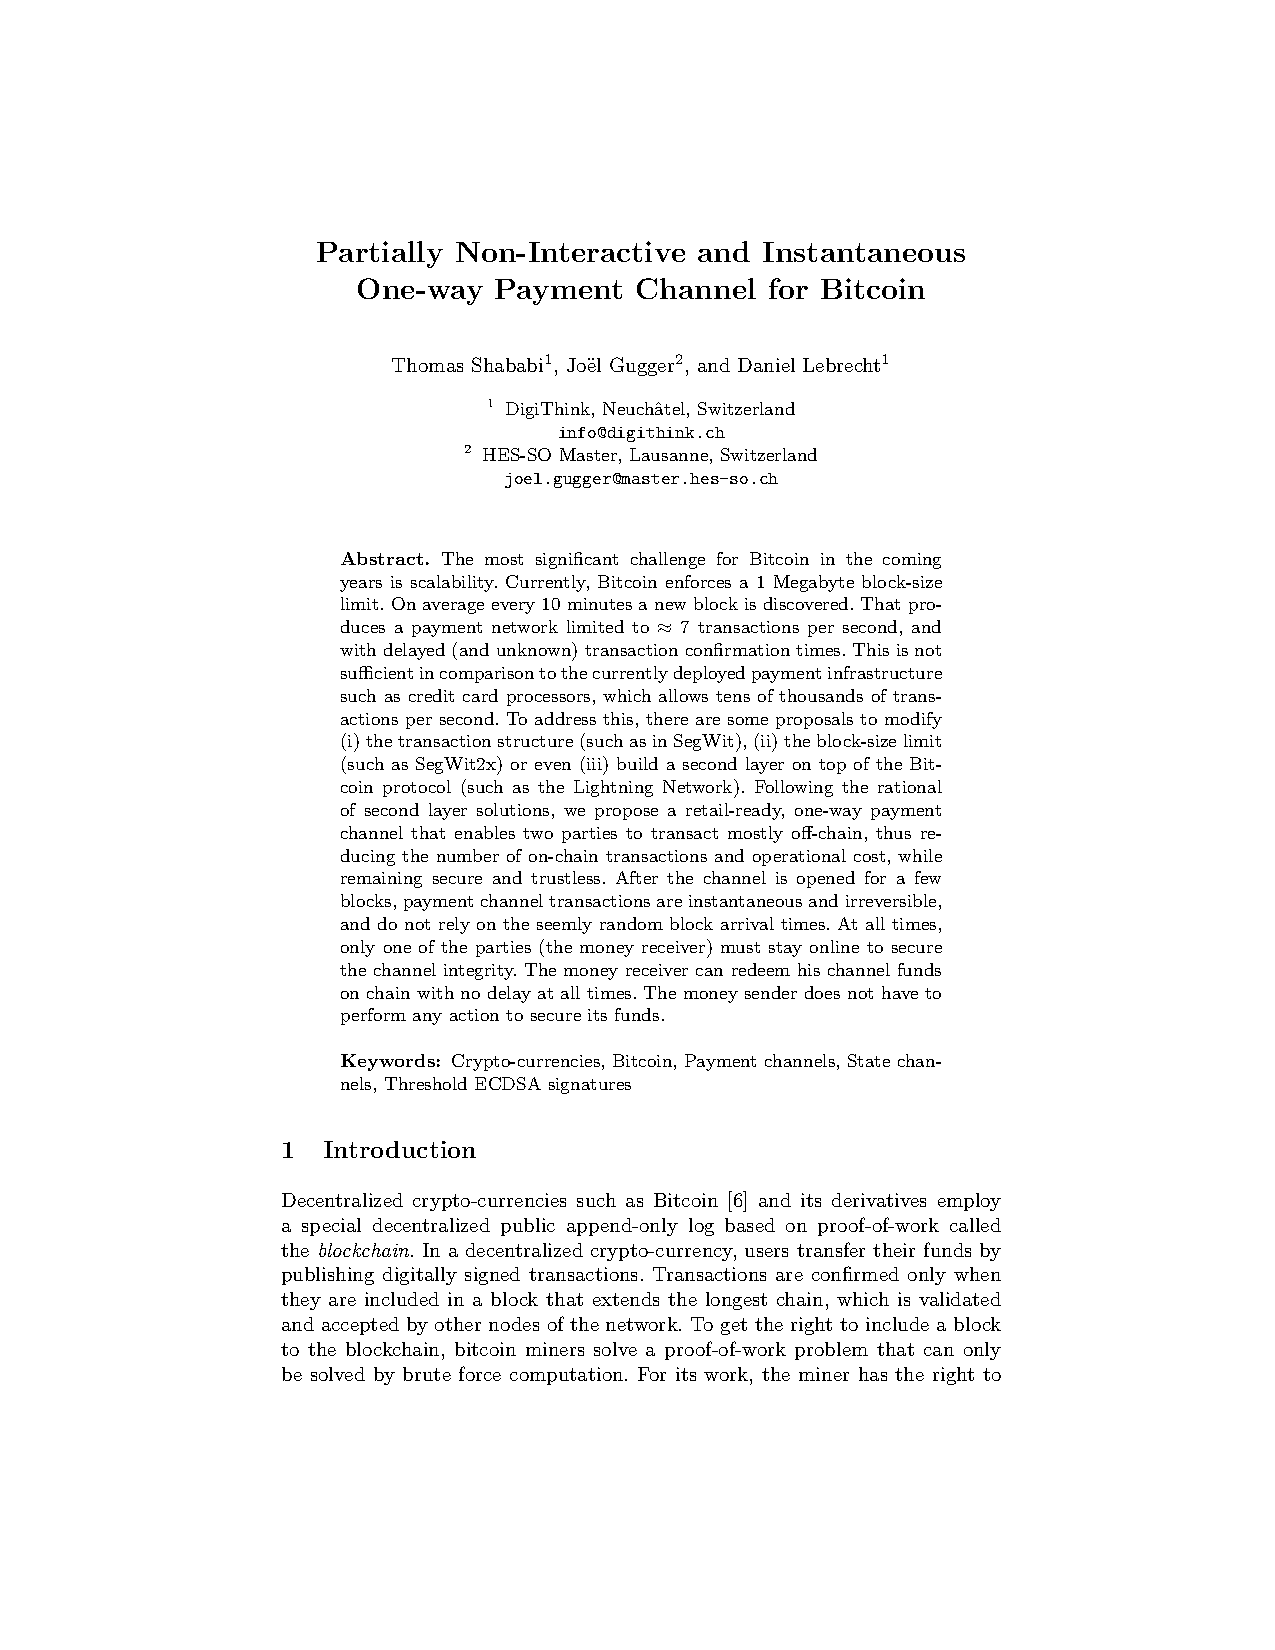
\includepdf[pages=-, addtotoc={1, chapter, 1, {One-way Payment Channel for Bitcoin}, chap:btcwp}]
  {03-tail/appendix/btc-channel.pdf}

% List of figures
\newpage\phantom{blank}
\thispagestyle{empty}
\cleardoublepage
\phantomsection
\addcontentsline{toc}{chapter}{List of Figures}
\listoffigures

% List of tables
\cleardoublepage
\phantomsection
\addcontentsline{toc}{chapter}{List of Tables}
\listoftables

% List of listings
\cleardoublepage
\phantomsection
\addcontentsline{toc}{chapter}{List of Sources}
\listoflistings

% -----------------------------------------------------------------------------
% Back matter
% -----------------------------------------------------------------------------
\backmatter

% Bibliography
\cleardoublepage

\printbibliography[heading=bibintoc]

% Glossary
\cleardoublepage
\printglossaries

\end{document}
